\section{Conclusiones.}

\newpage

\section{Trabajos futuros.}

\section{Anexo: Vista de la aplicación web y instalación PWA.}

\subsection{Vista de la API.}

\begin{figure}[ht!]
  \centering
  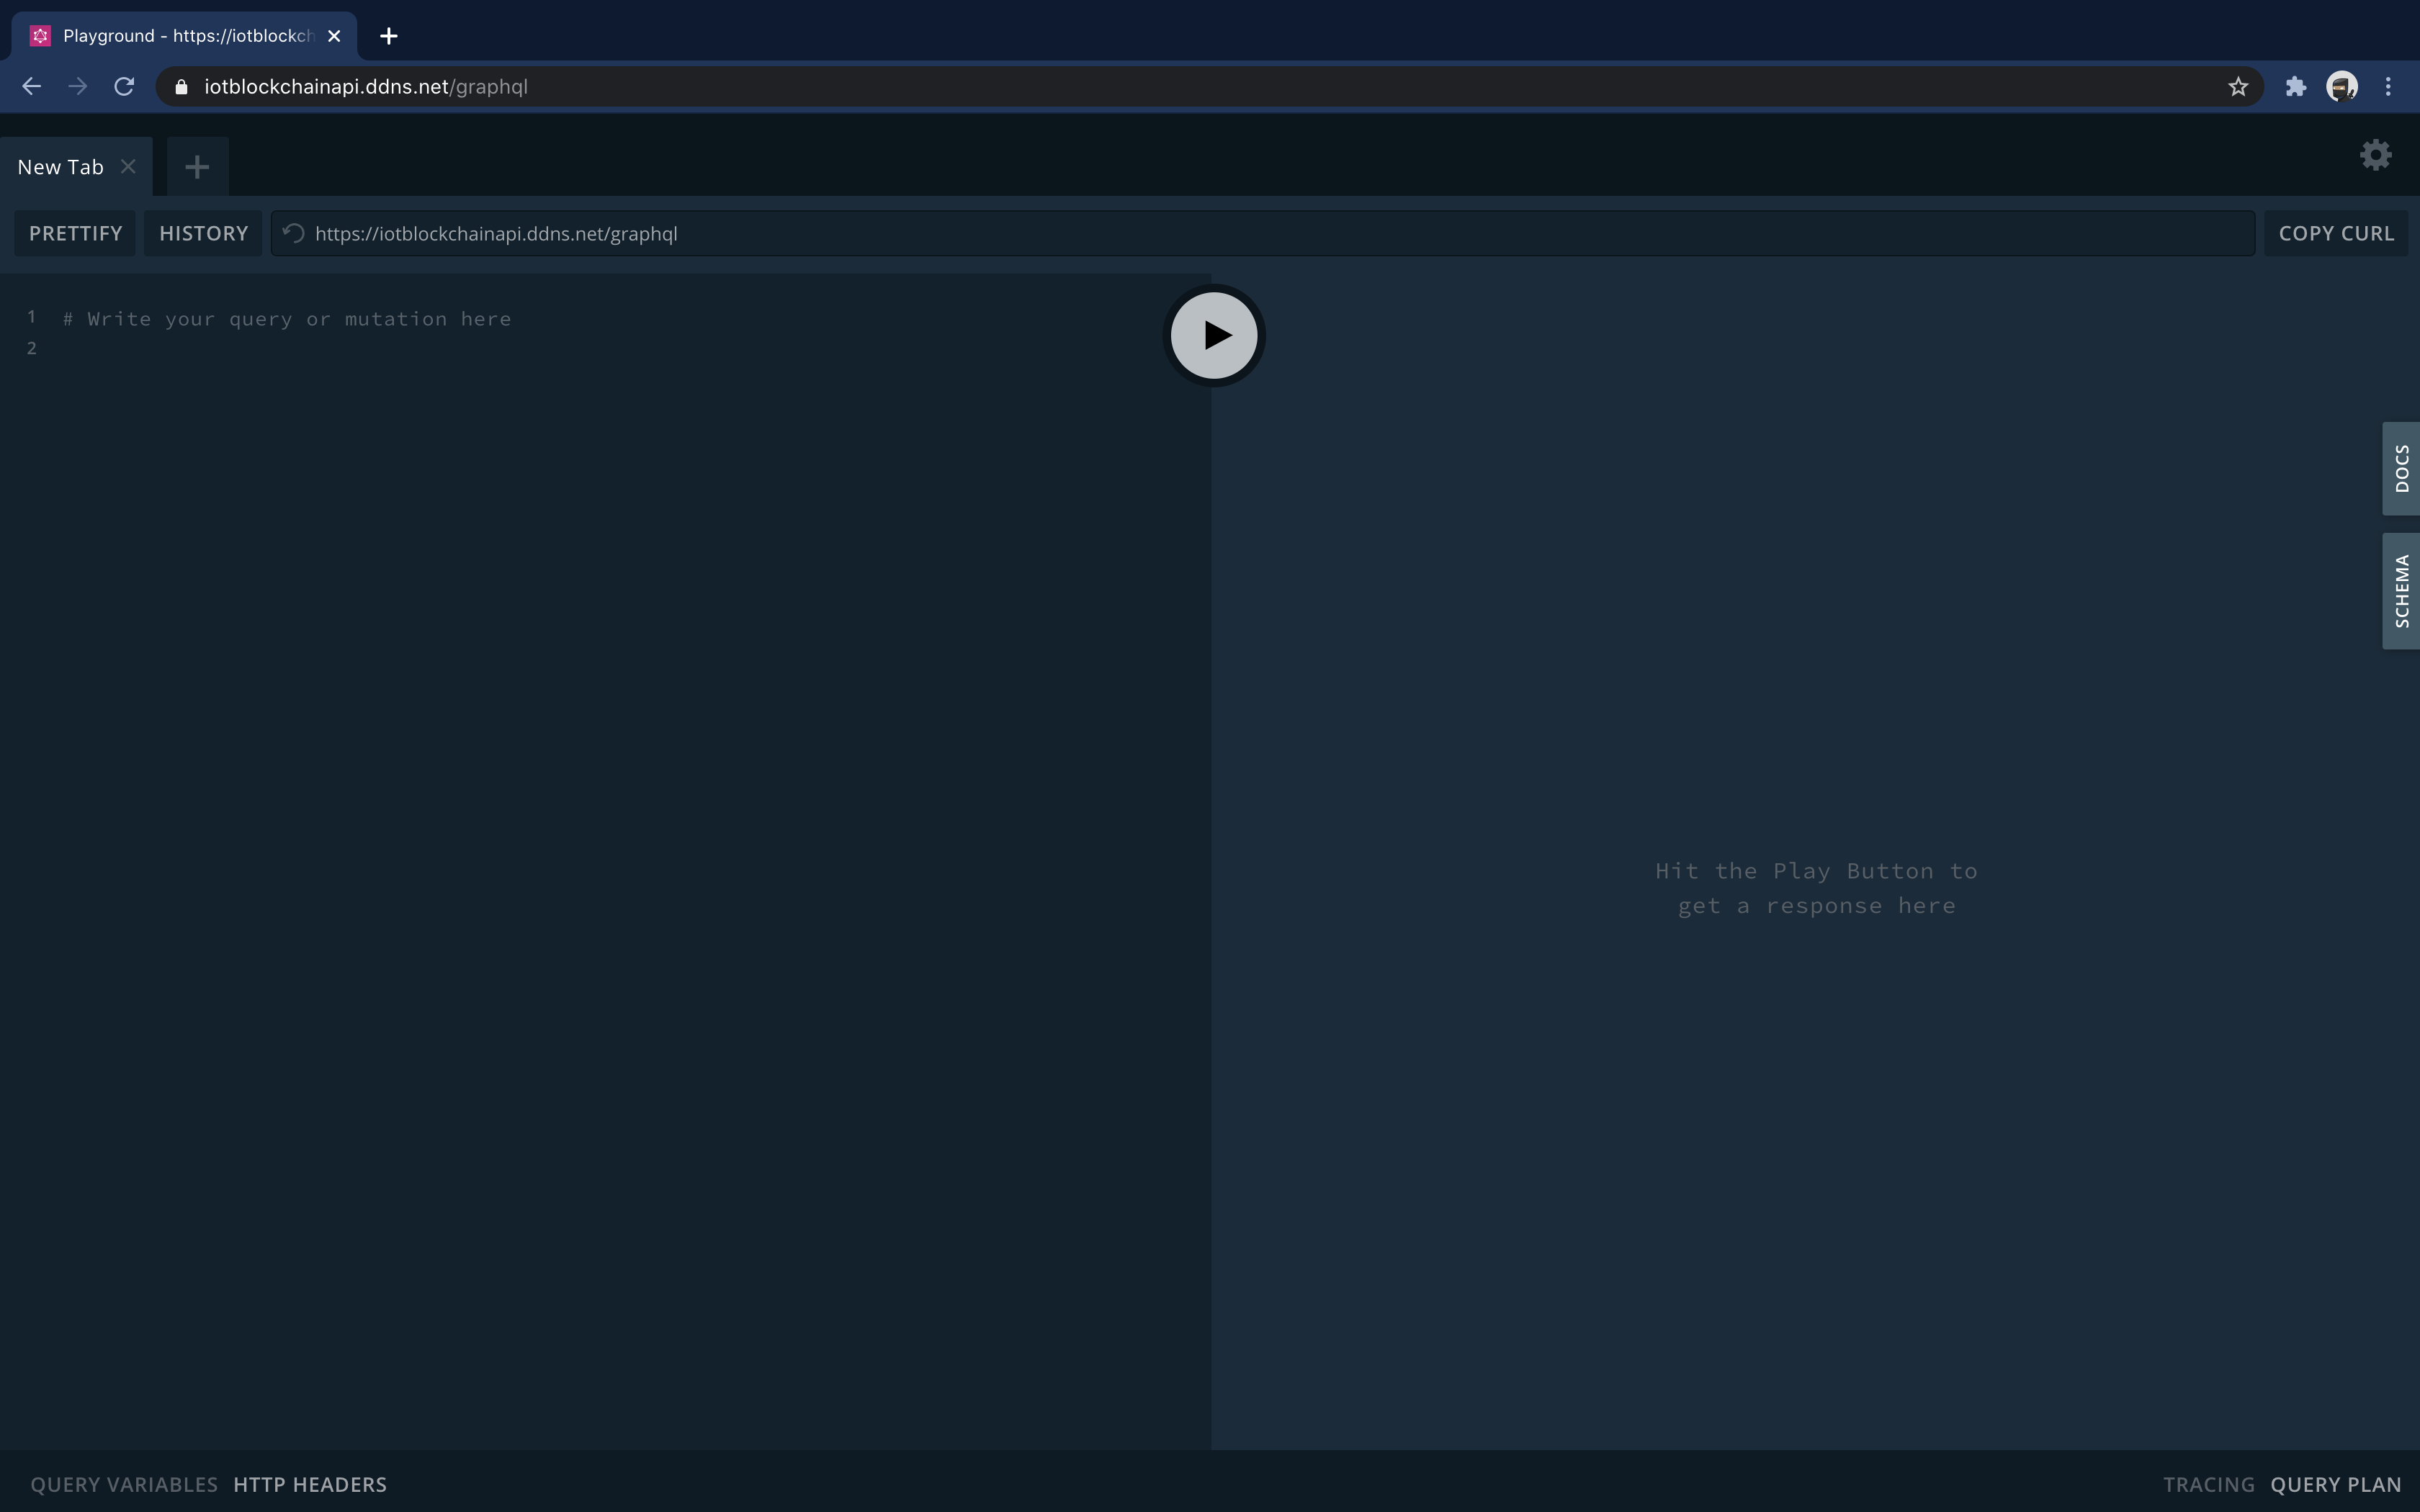
\includegraphics[width=10cm]{imagenes/desarrollo/web/api/graphql_api}
  \caption{GraphQL API endpoint.}
  \label{fig:graphql-api}
\end{figure}

\begin{figure}[ht!]
  \centering
  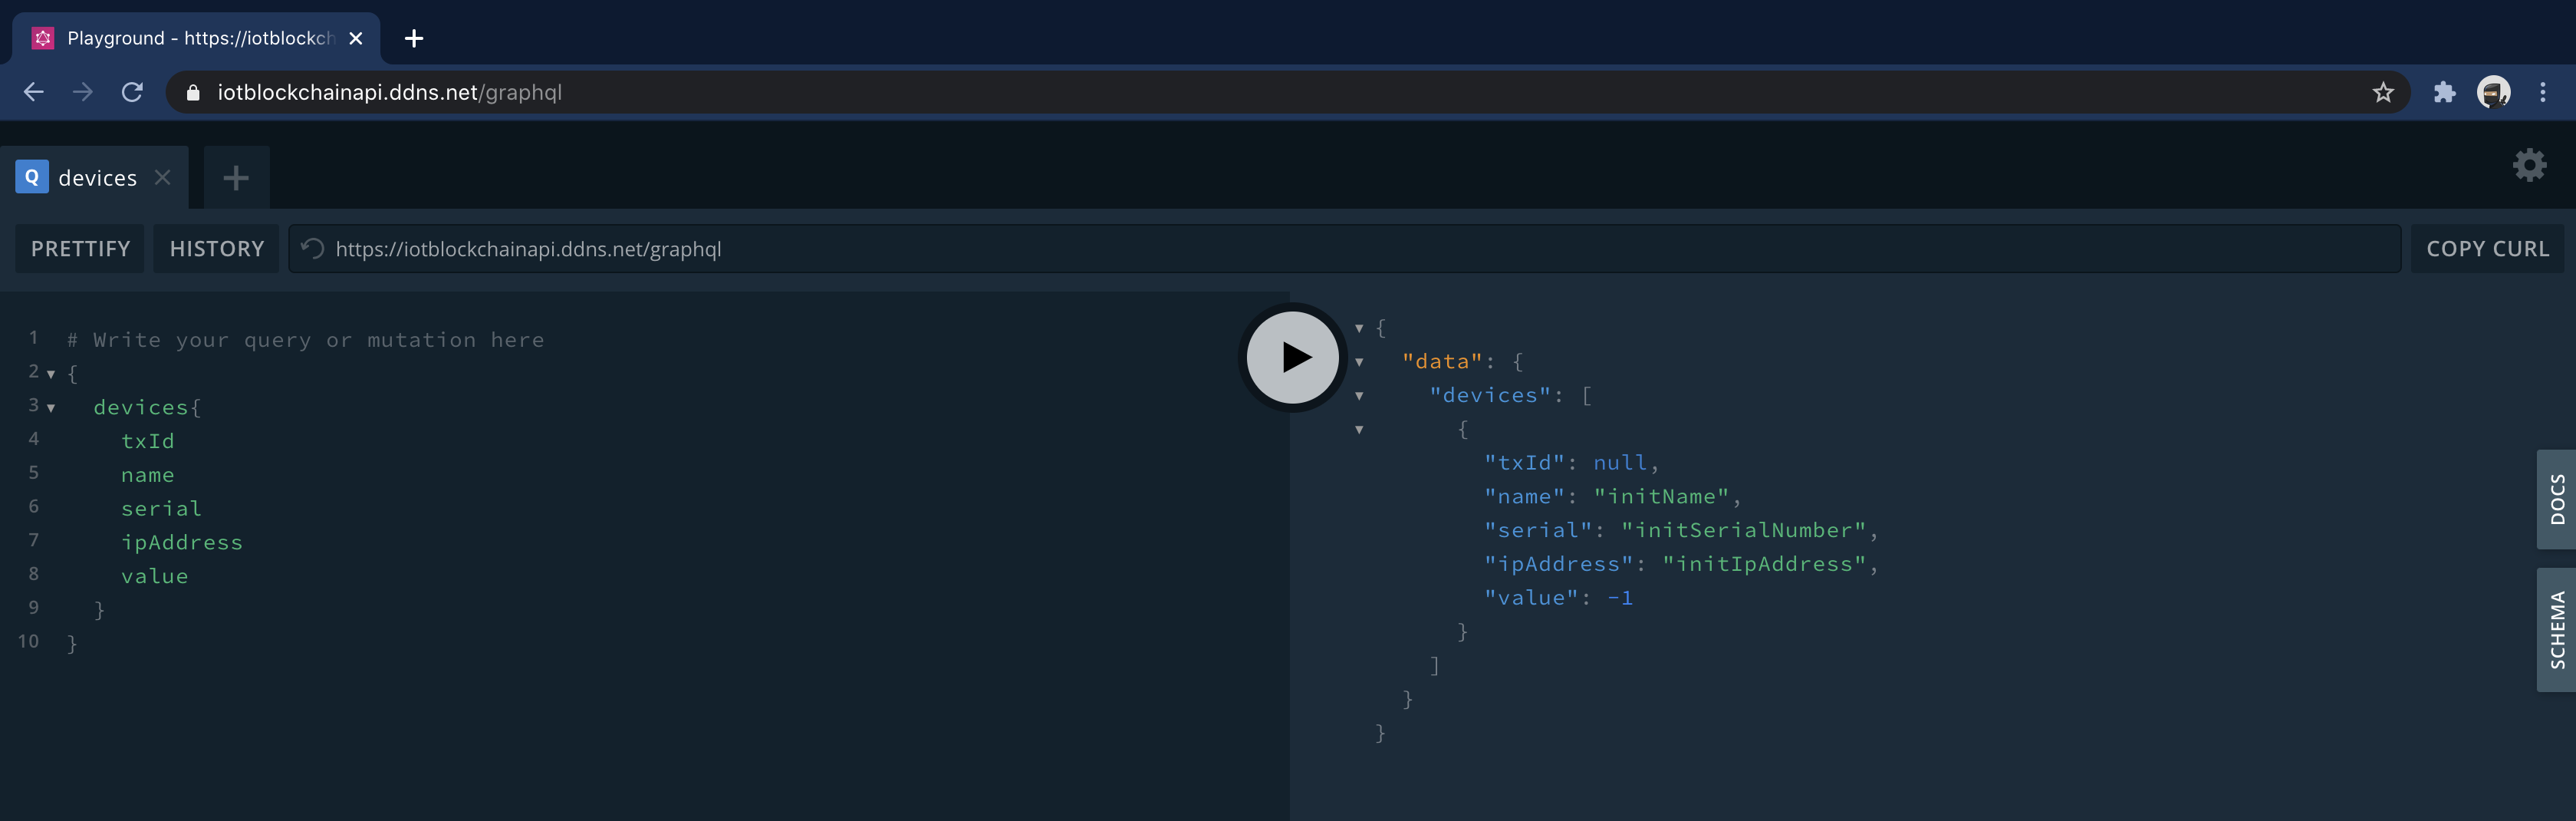
\includegraphics[width=10cm]{imagenes/desarrollo/web/api/graphql_query}
  \caption{Consulta a GraphQL API endpoint.}
  \label{fig:query-graphql-api}
\end{figure}

\begin{figure}[ht!]
  \centering
  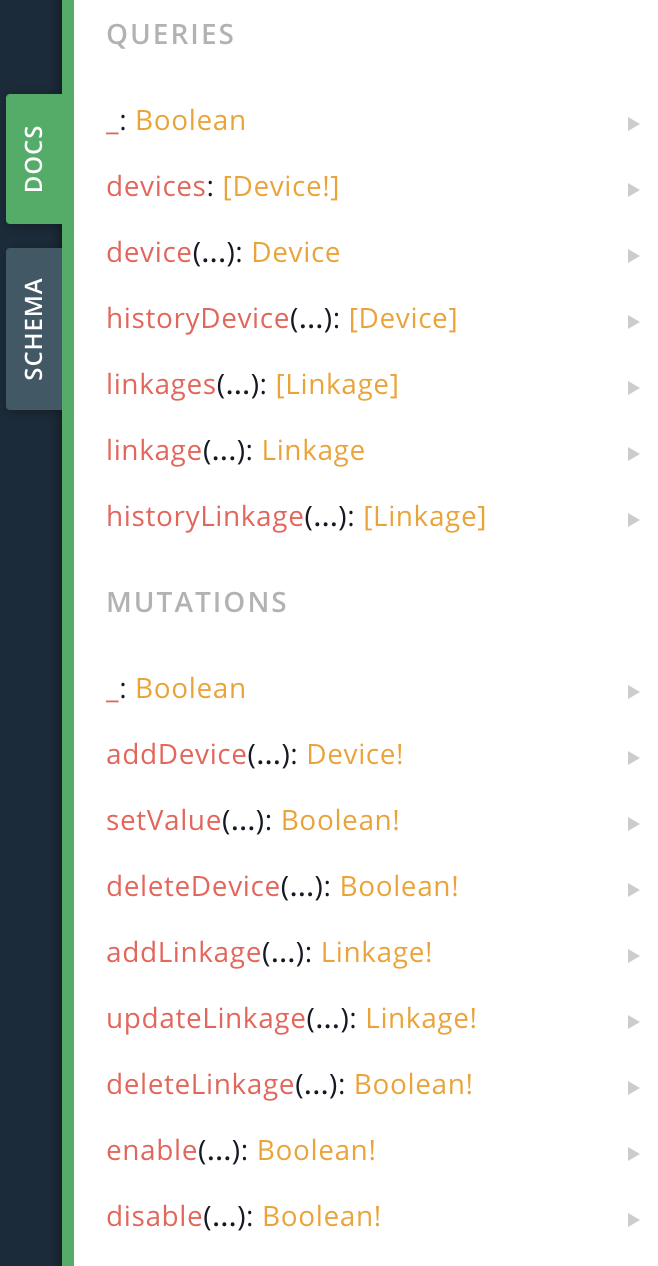
\includegraphics[width=10cm]{imagenes/desarrollo/web/api/graphql_docs}
  \caption{Docs GraphQL API.}
  \label{fig:graphql-docs}
\end{figure}

\begin{figure}[ht!]
  \centering
  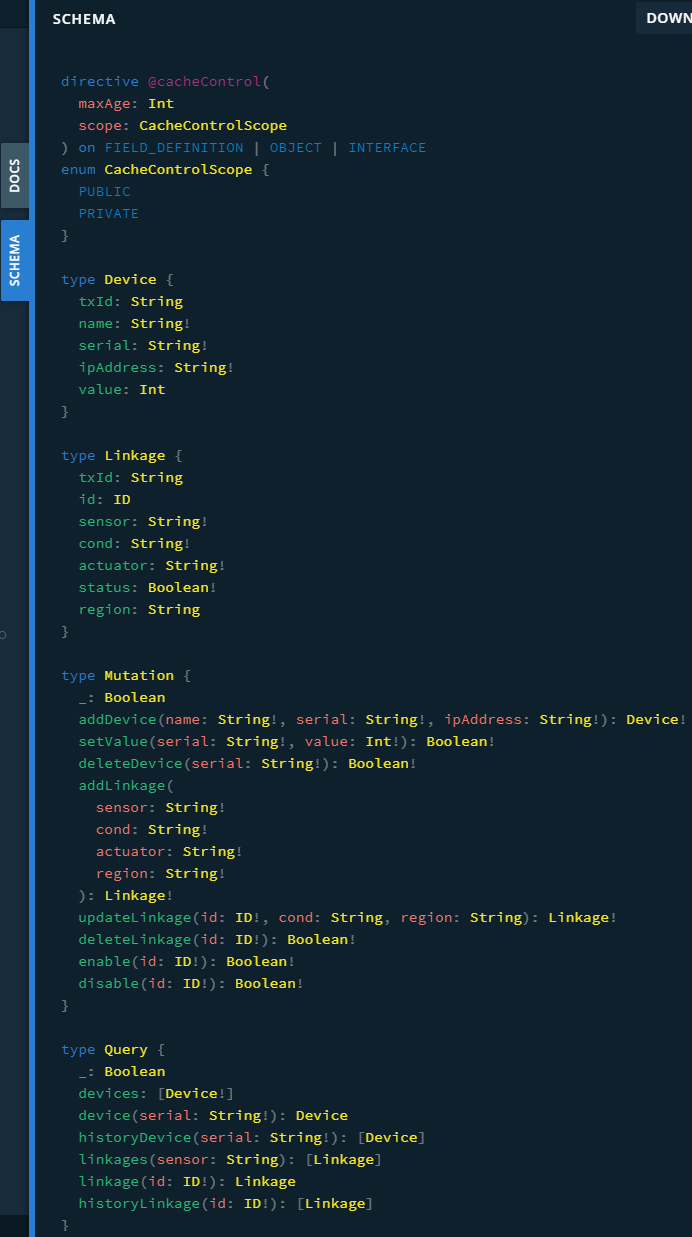
\includegraphics[width=10cm]{imagenes/desarrollo/web/api/graphql_schema}
  \caption{Schema GraphQL API.}
  \label{fig:graphql-schema}
\end{figure}

\subsection{Vista del Frontend.}

\begin{figure}[ht!]
  \centering
  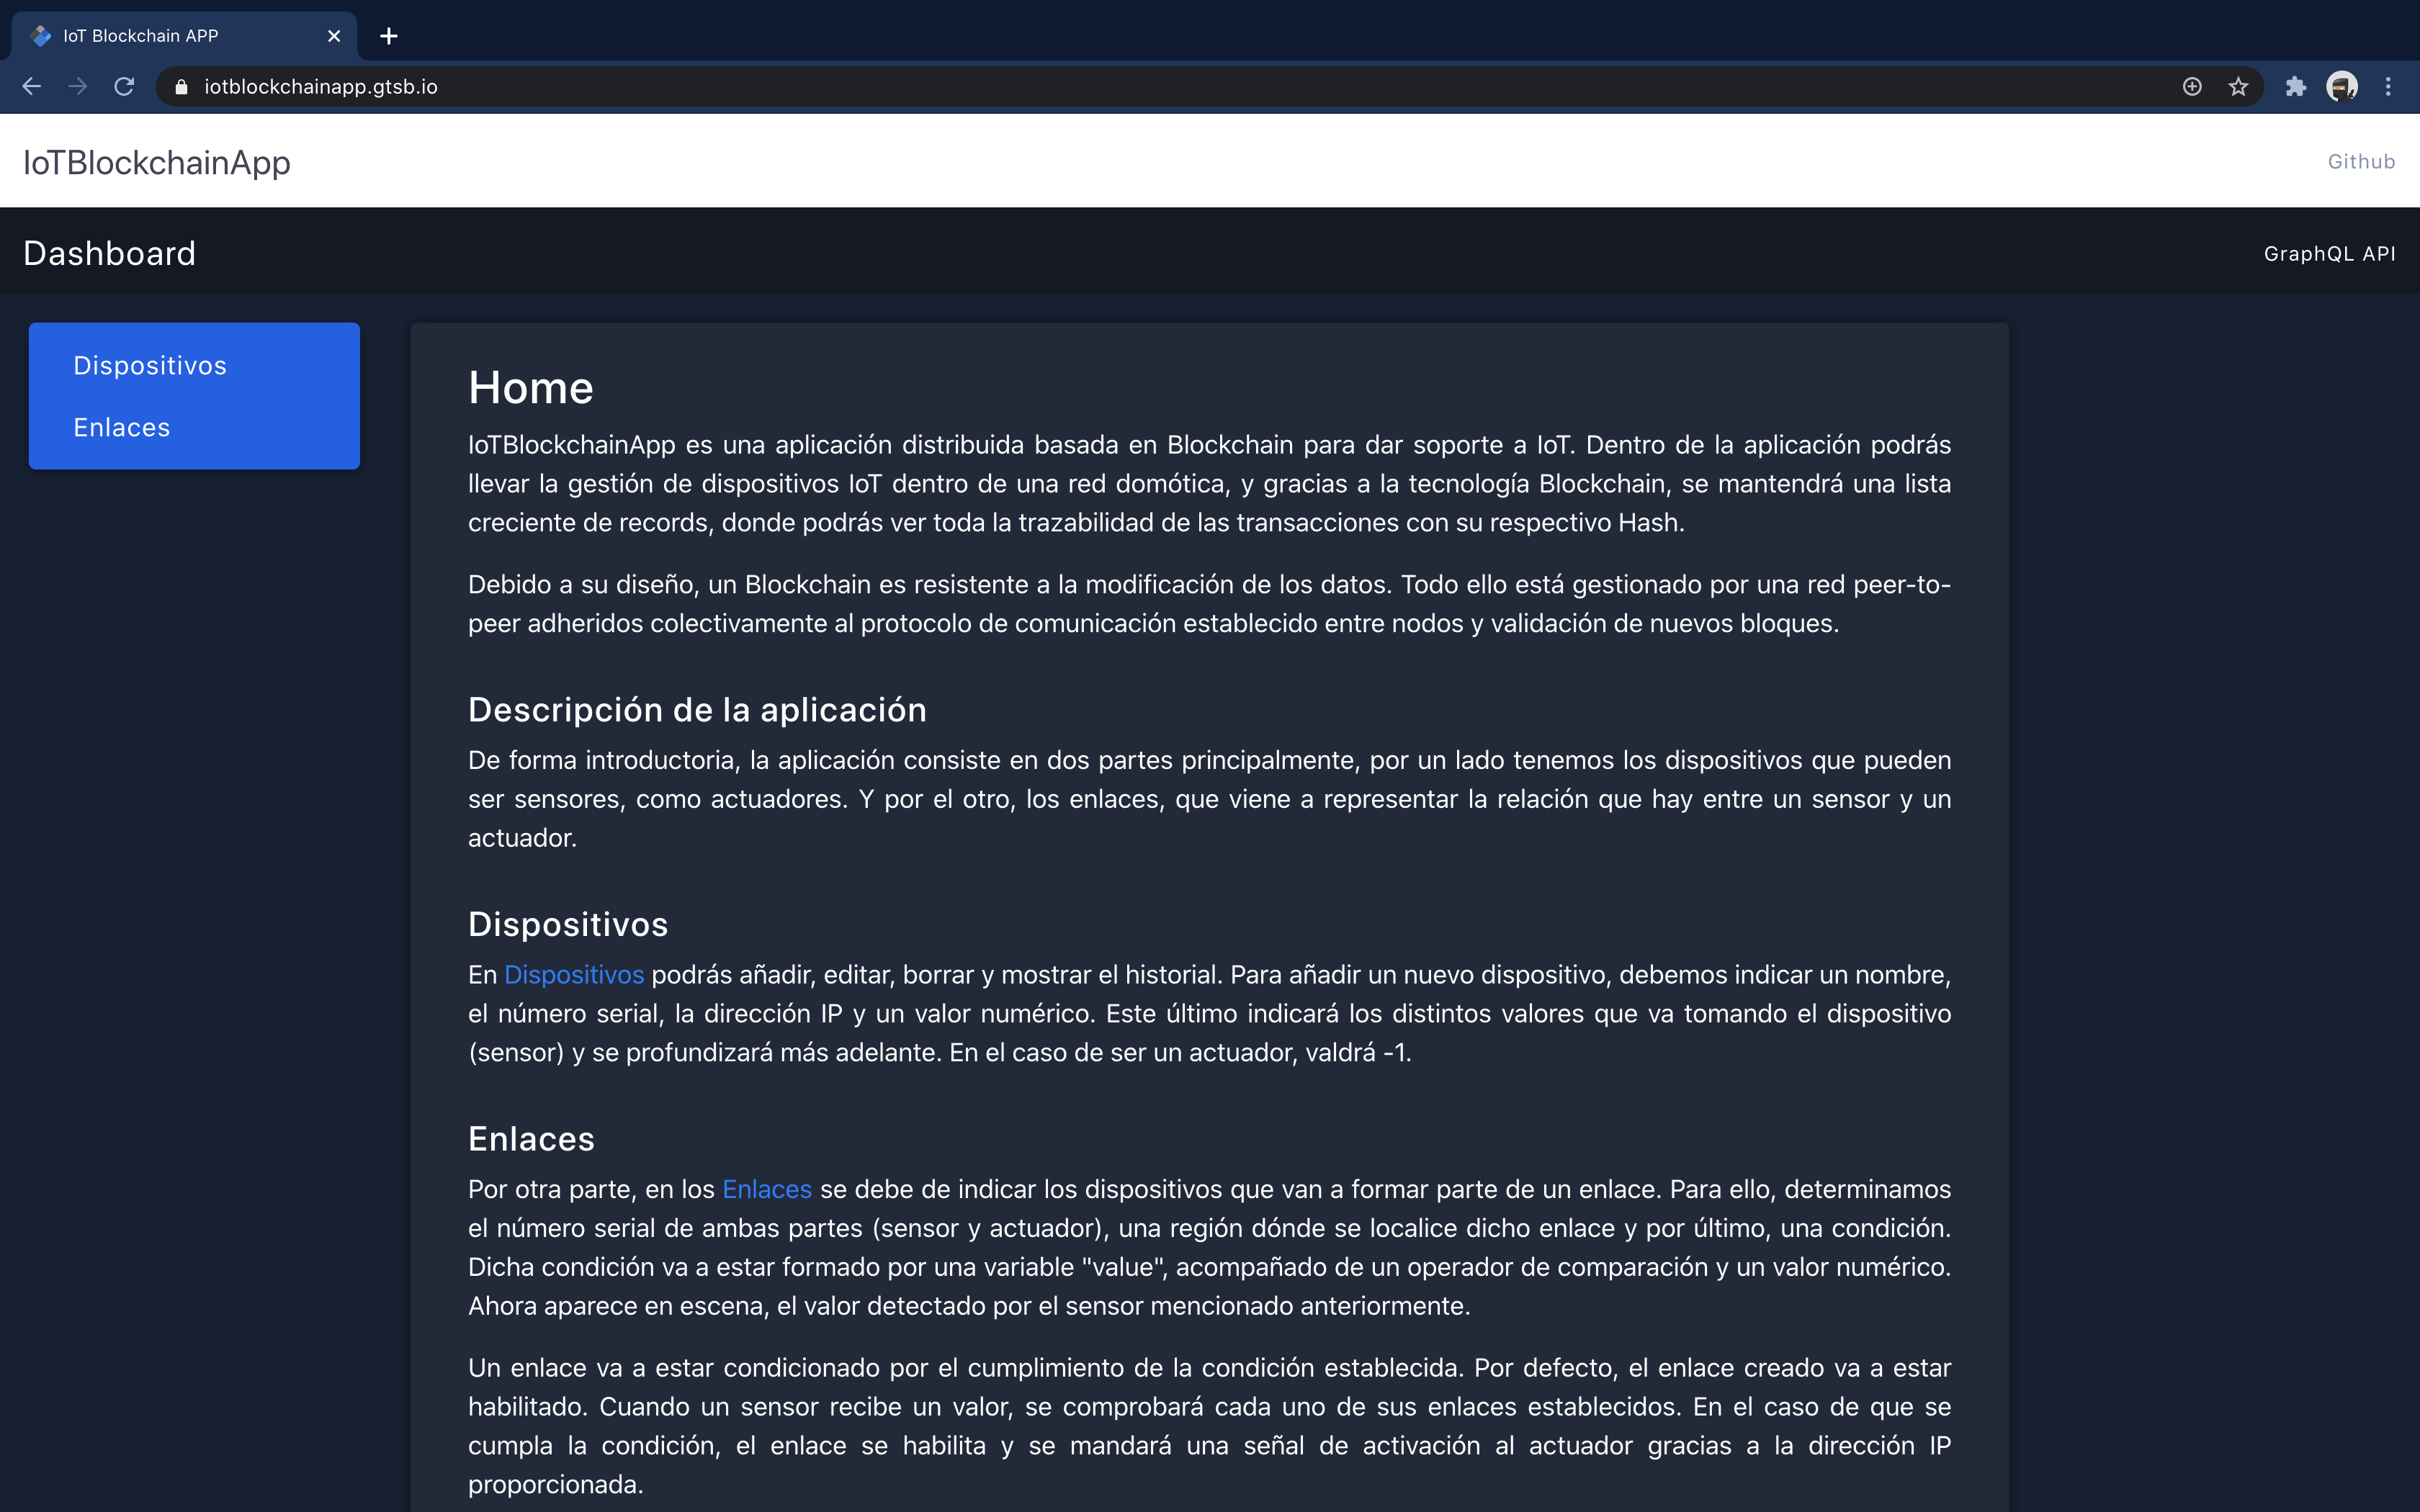
\includegraphics[width=10cm]{imagenes/desarrollo/web/pagina_inicial}
  \caption{Página inicial.}
  \label{fig:pagina-inicial}
\end{figure}

\subsubsection*{Vista dispositivo.}

\begin{figure}[ht!]
  \centering
  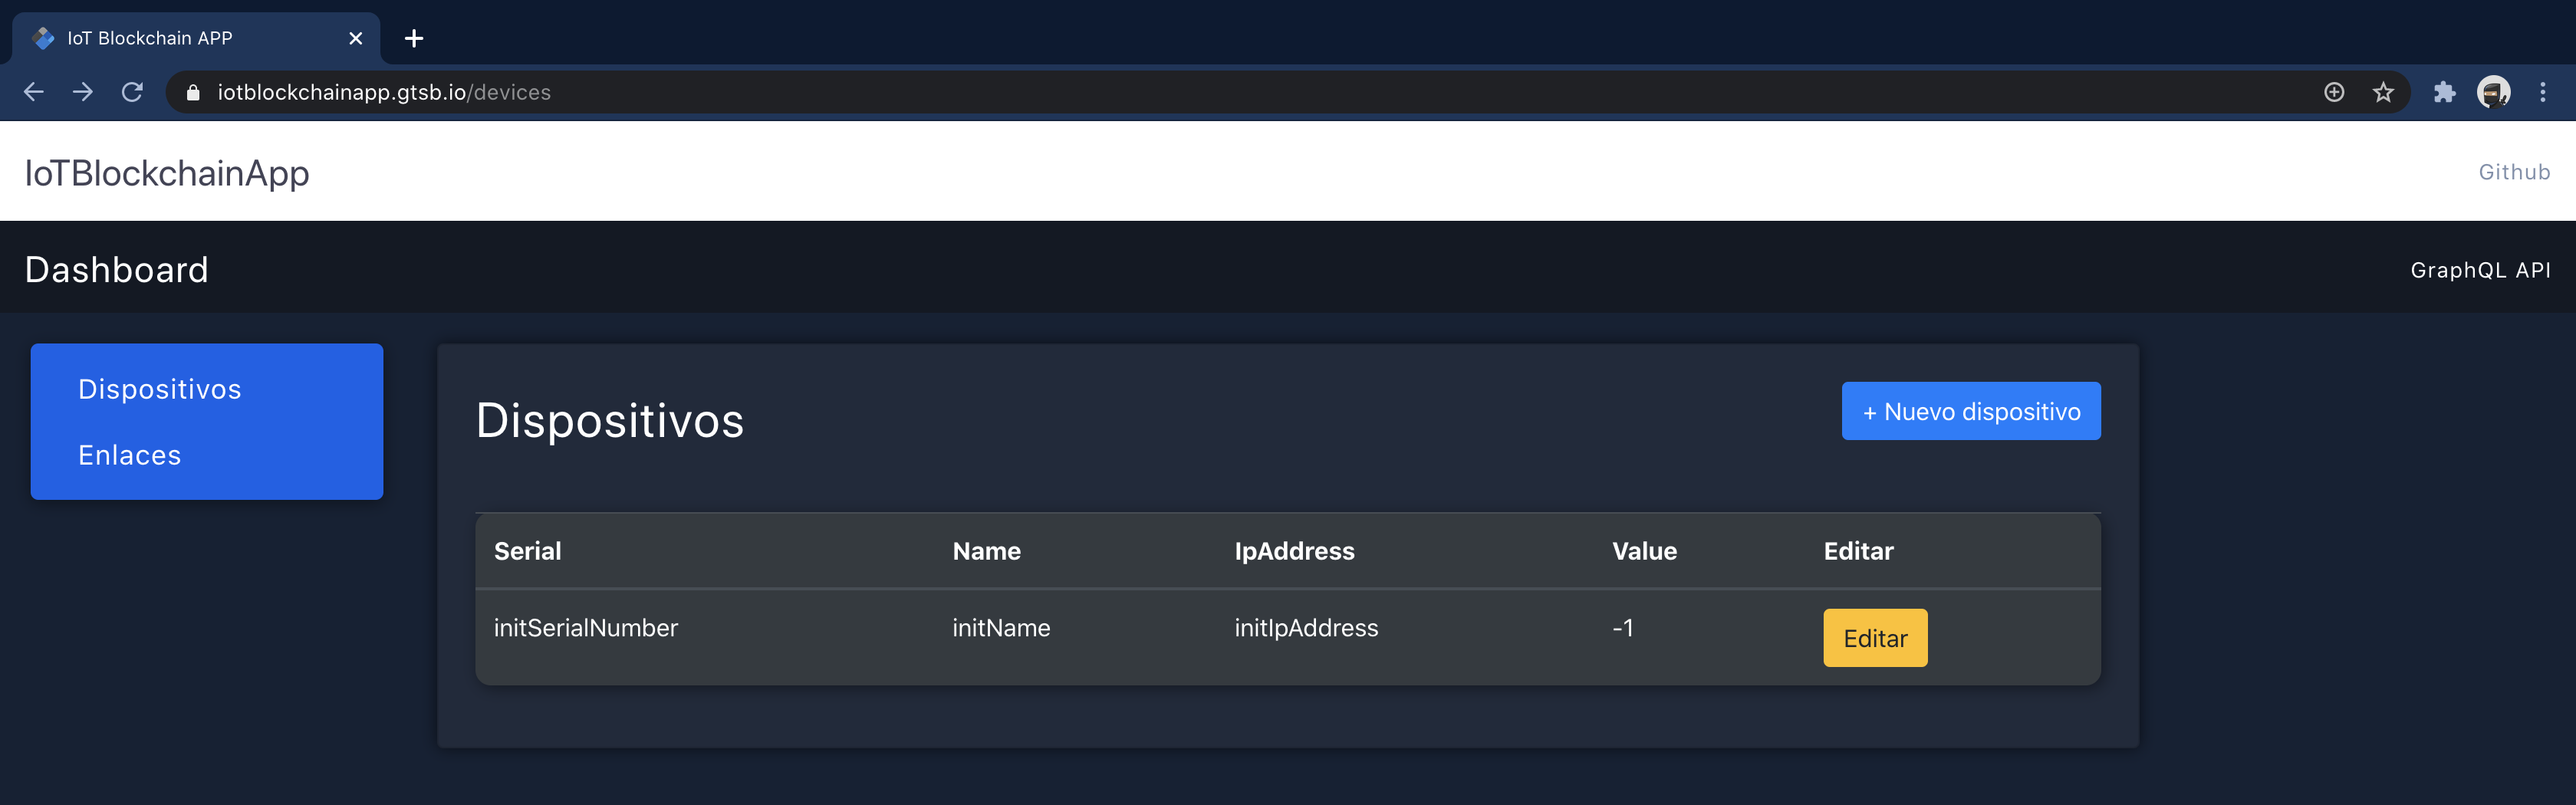
\includegraphics[width=10cm]{imagenes/desarrollo/web/vista_dispositivos}
  \caption{Vista dispositivos.}
  \label{fig:vista-dispositivo}
\end{figure}

\begin{figure}[ht!]
  \centering
  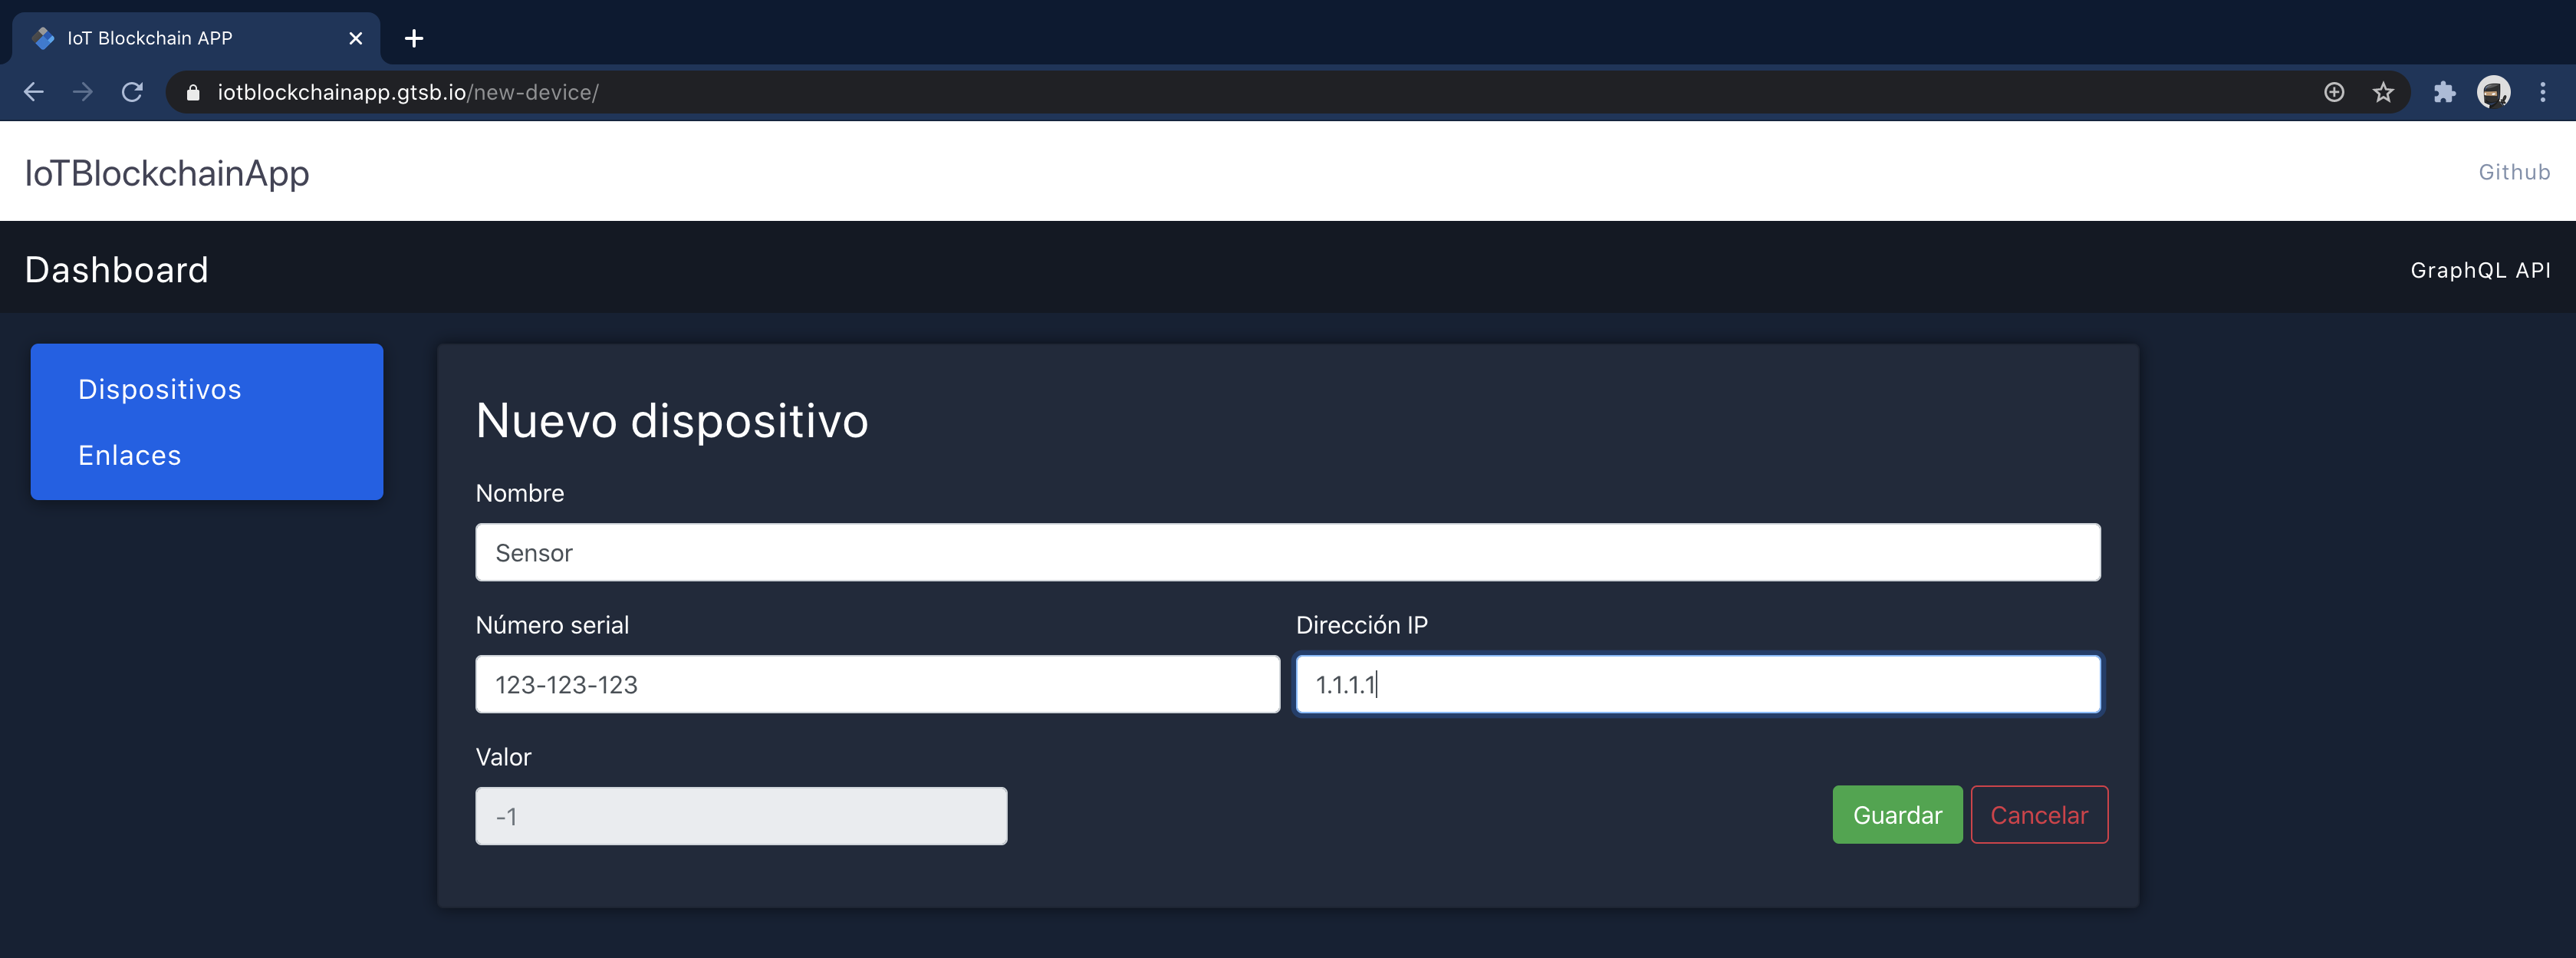
\includegraphics[width=10cm]{imagenes/desarrollo/web/aniadir_dispositivo}
  \caption{Añadir dispositivo.}
  \label{fig:aniadir-dispositivo}
\end{figure}

\begin{figure}[ht!]
  \centering
  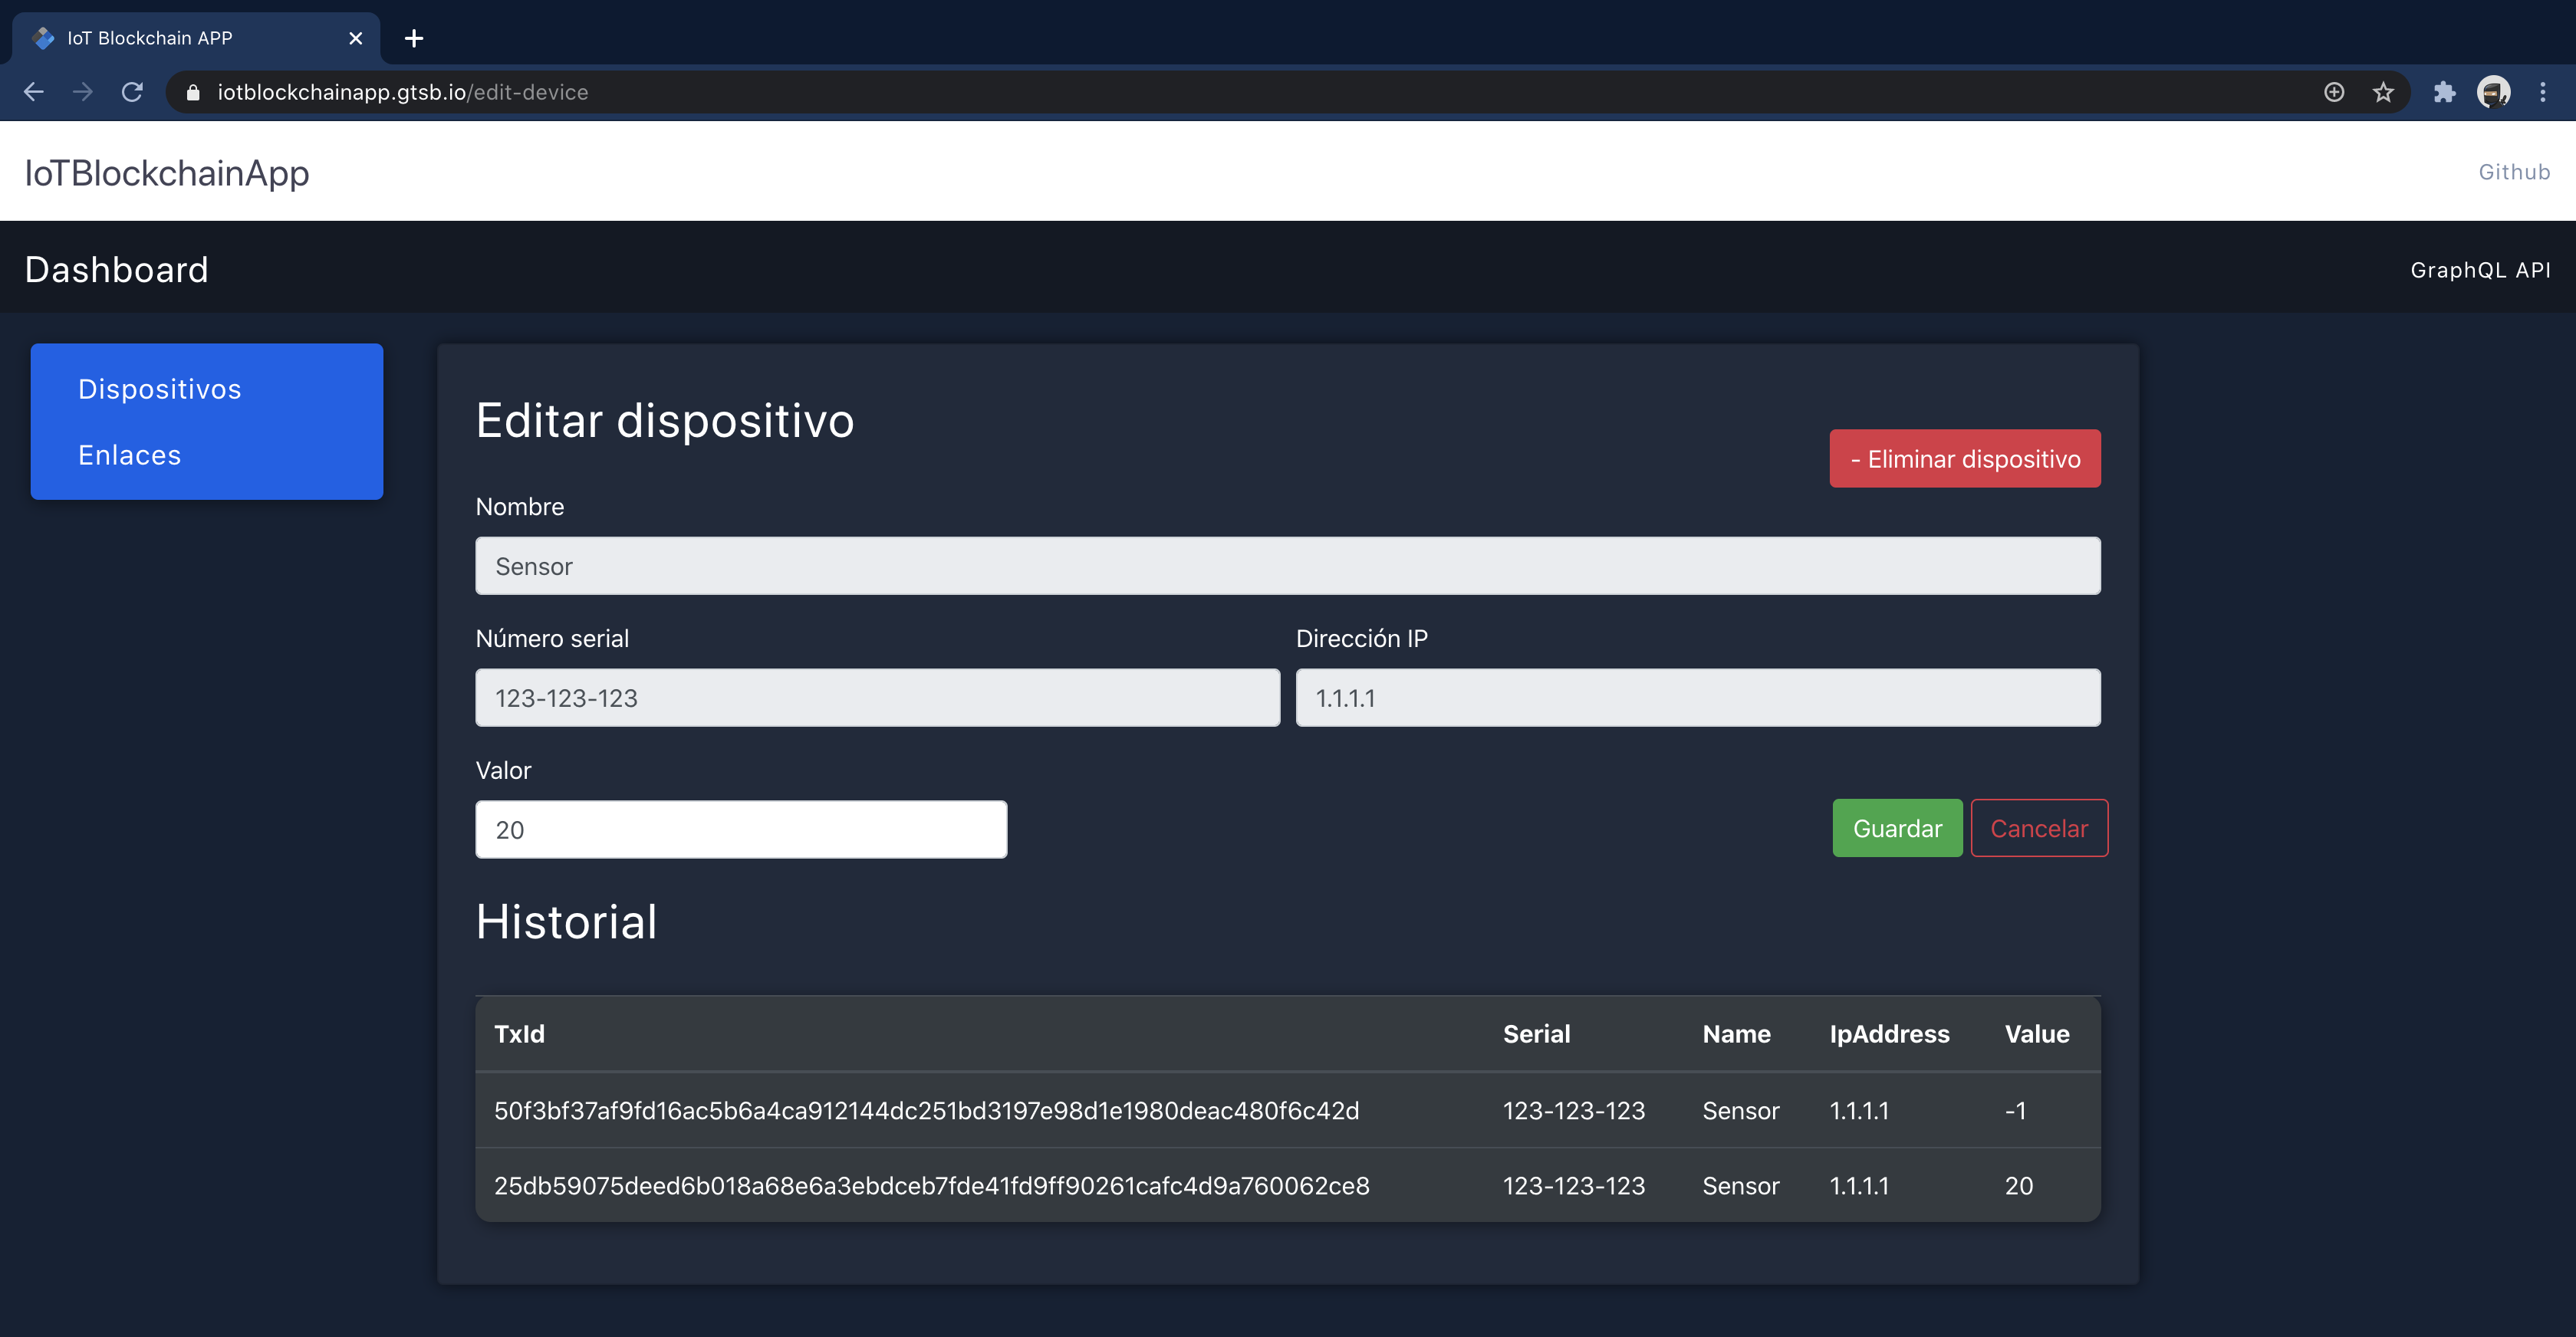
\includegraphics[width=10cm]{imagenes/desarrollo/web/editar_dispositivo}
  \caption{Editar dispositivo.}
  \label{fig:editar-dispositivo}
\end{figure}

\subsubsection*{Vista enlace.}

\begin{figure}[ht!]
  \centering
  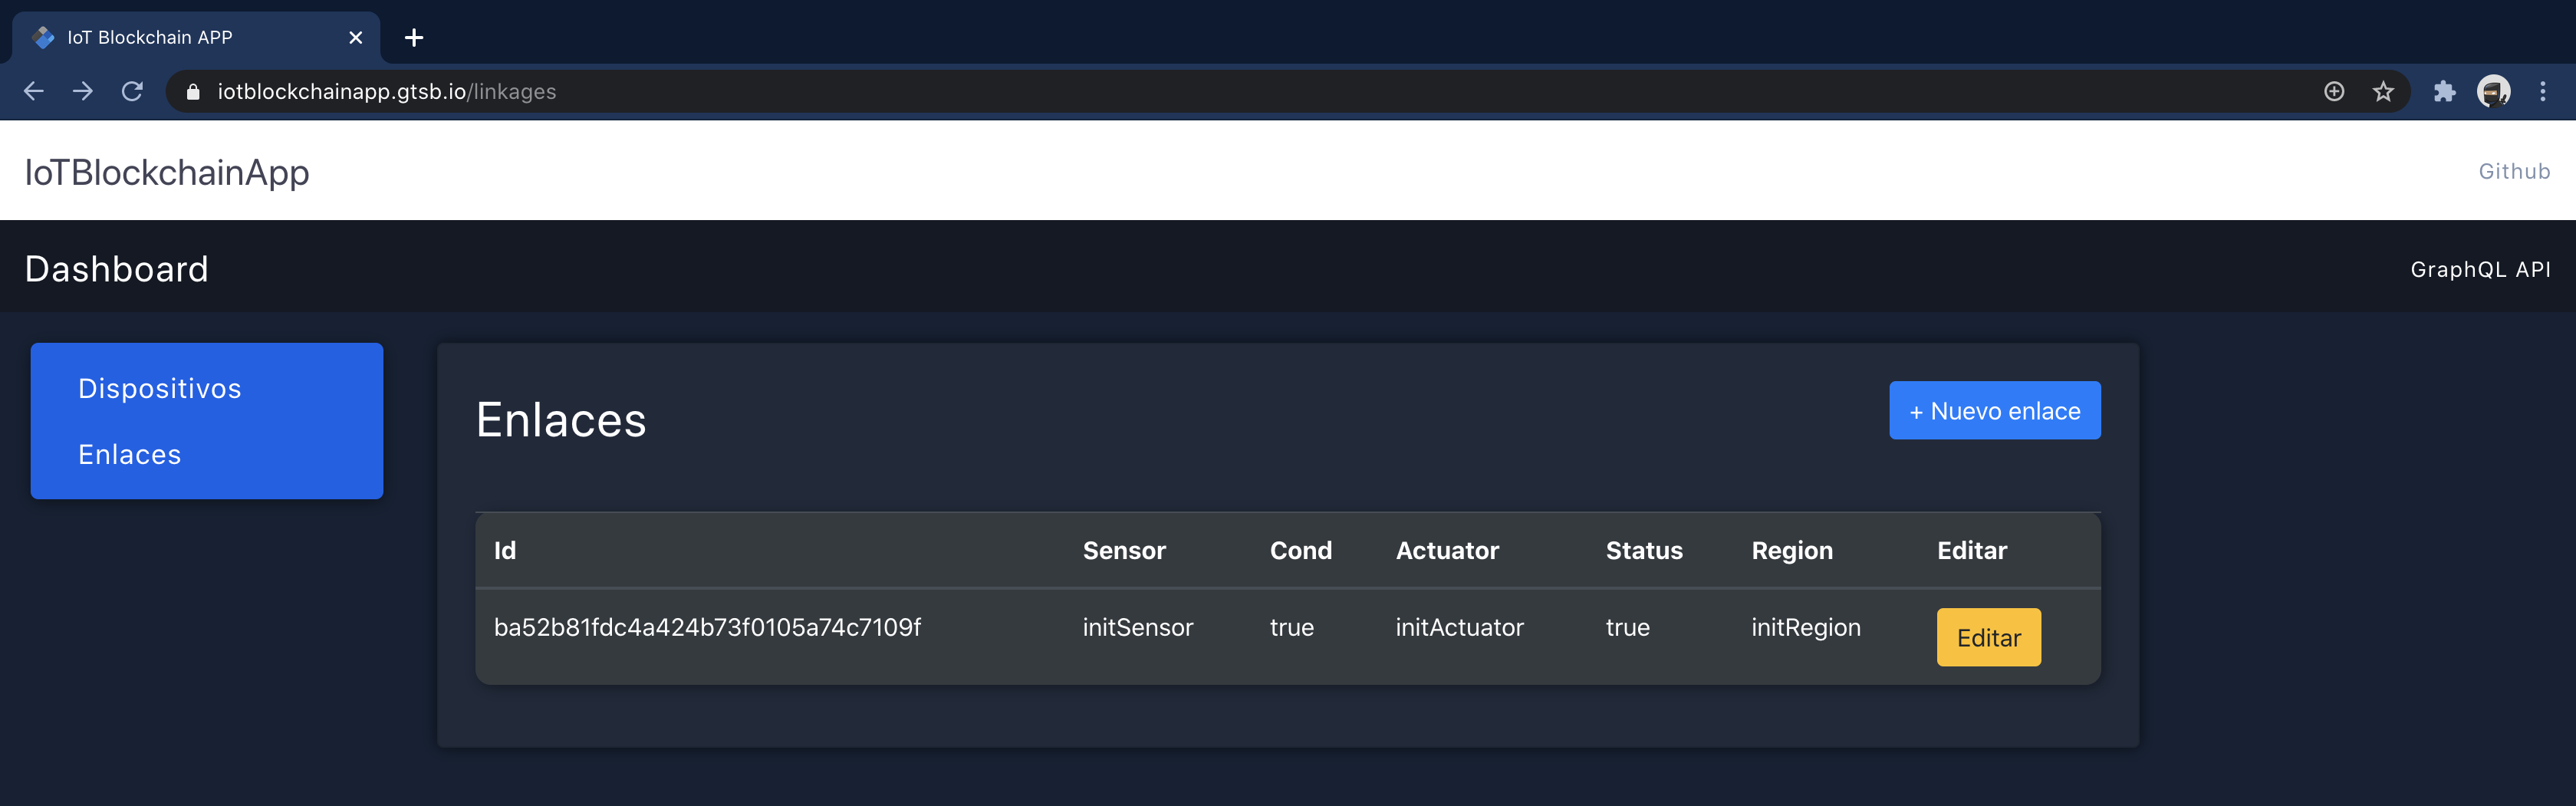
\includegraphics[width=10cm]{imagenes/desarrollo/web/vista_enlaces}
  \caption{Vista enlaces.}
  \label{fig:vista-enlace}
\end{figure}

\begin{figure}[ht!]
  \centering
  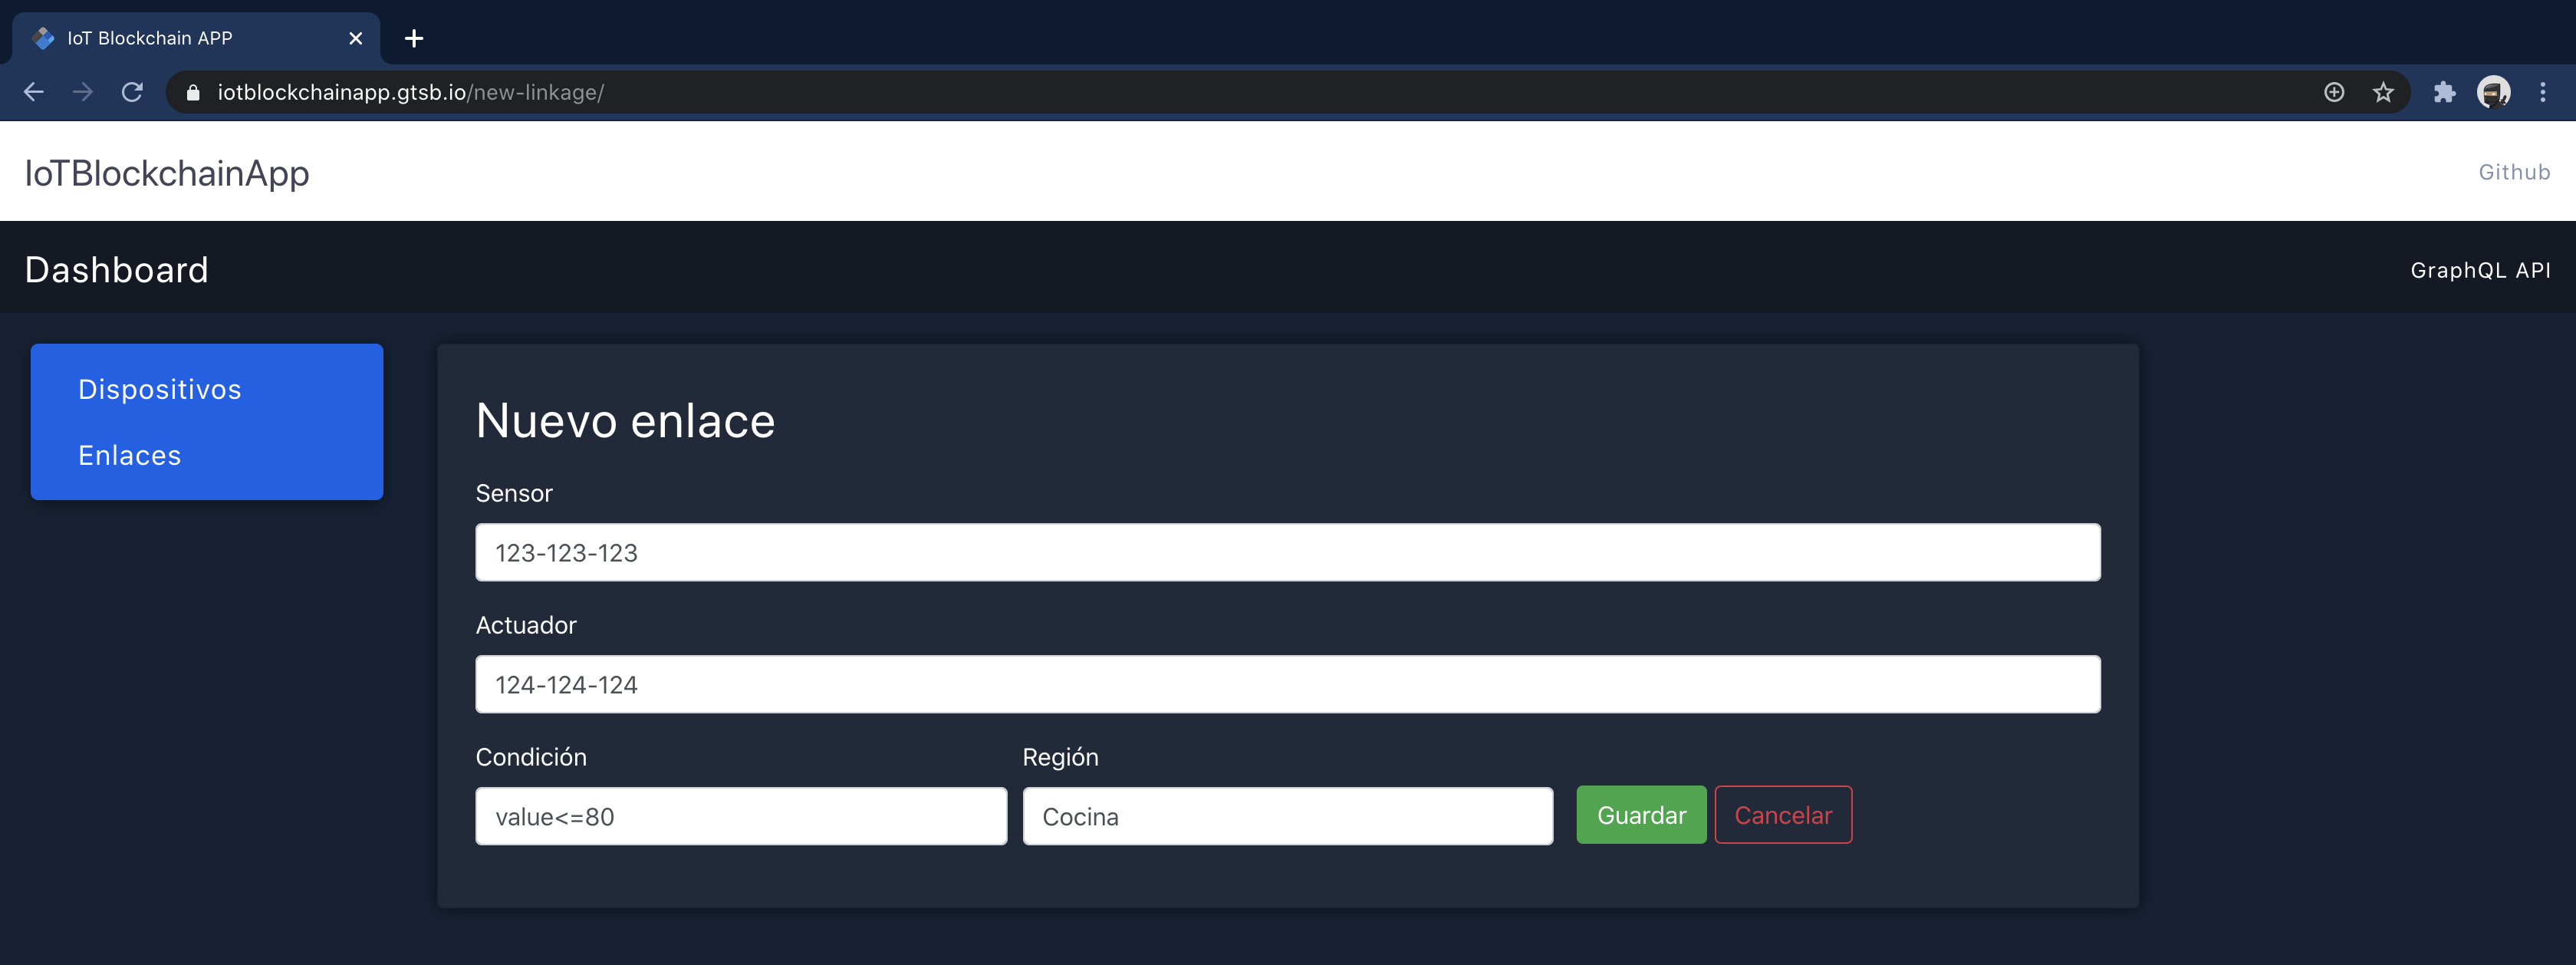
\includegraphics[width=10cm]{imagenes/desarrollo/web/aniadir_enlace}
  \caption{Añadir enlace.}
  \label{fig:aniadir-enlace}
\end{figure}

\begin{figure}[ht!]
  \centering
  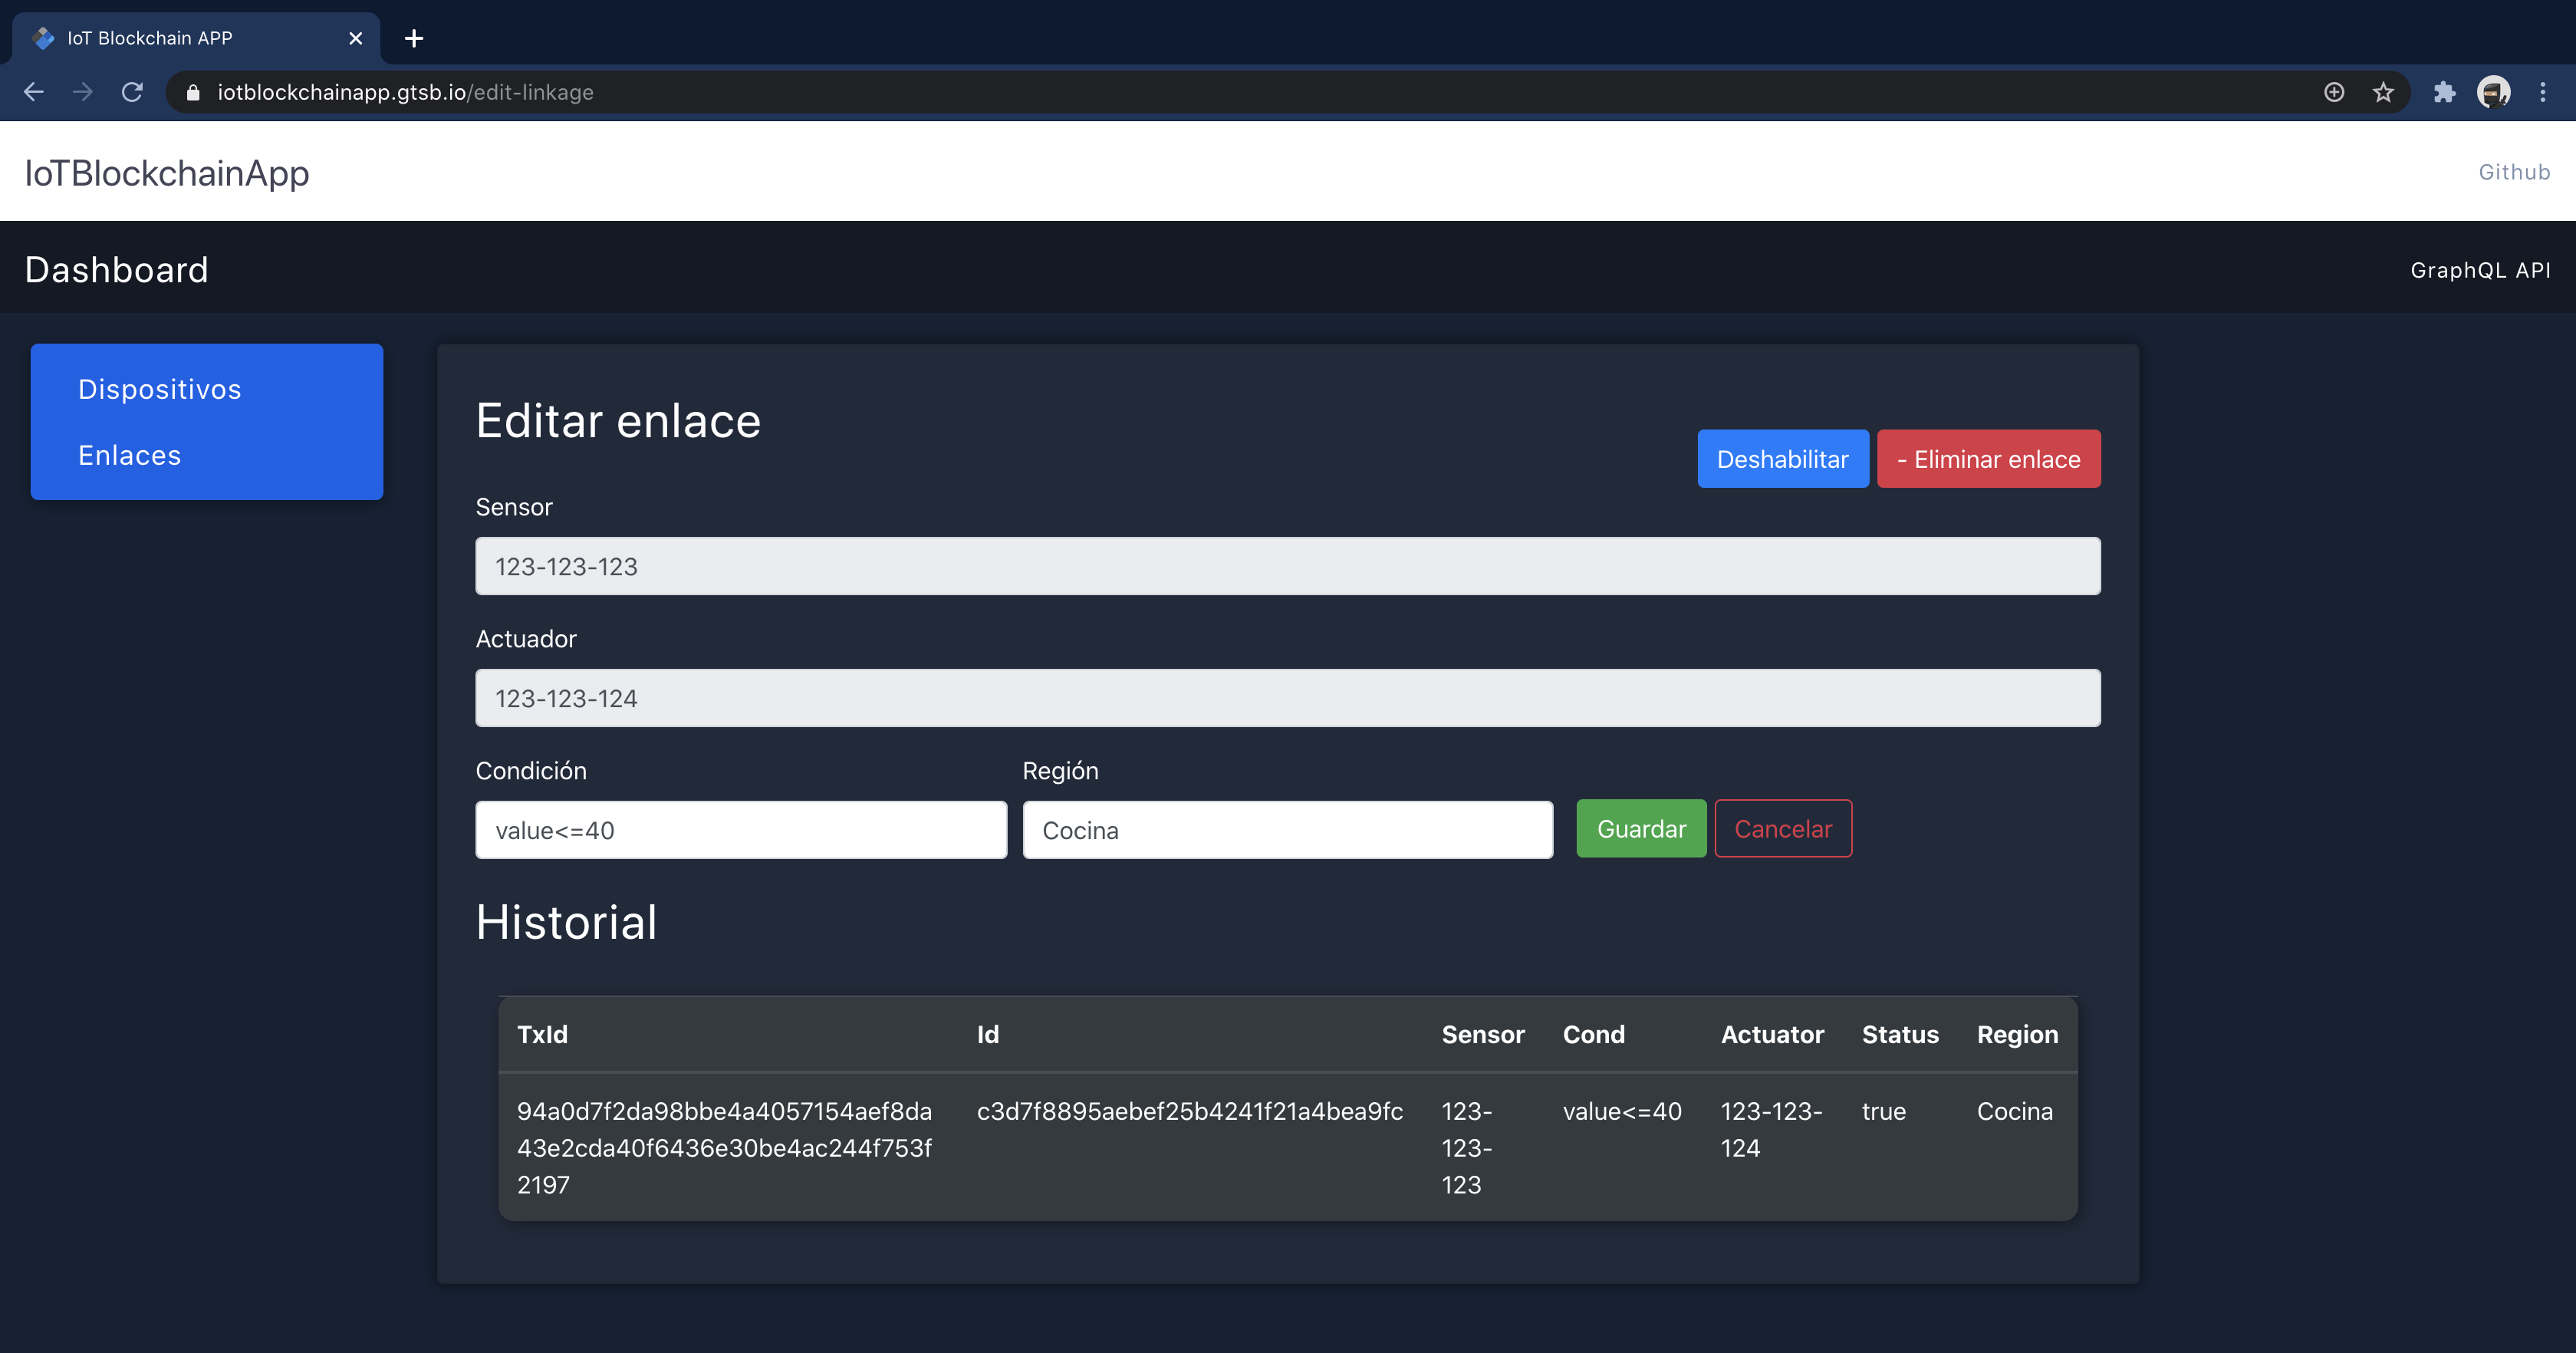
\includegraphics[width=10cm]{imagenes/desarrollo/web/editar_enlace}
  \caption{Editar enlace.}
  \label{fig:editar-enlace}
\end{figure}

\subsection{Instalación de PWA.}

\subsubsection*{Portatil.}

\begin{figure}[ht!]
  \centering
  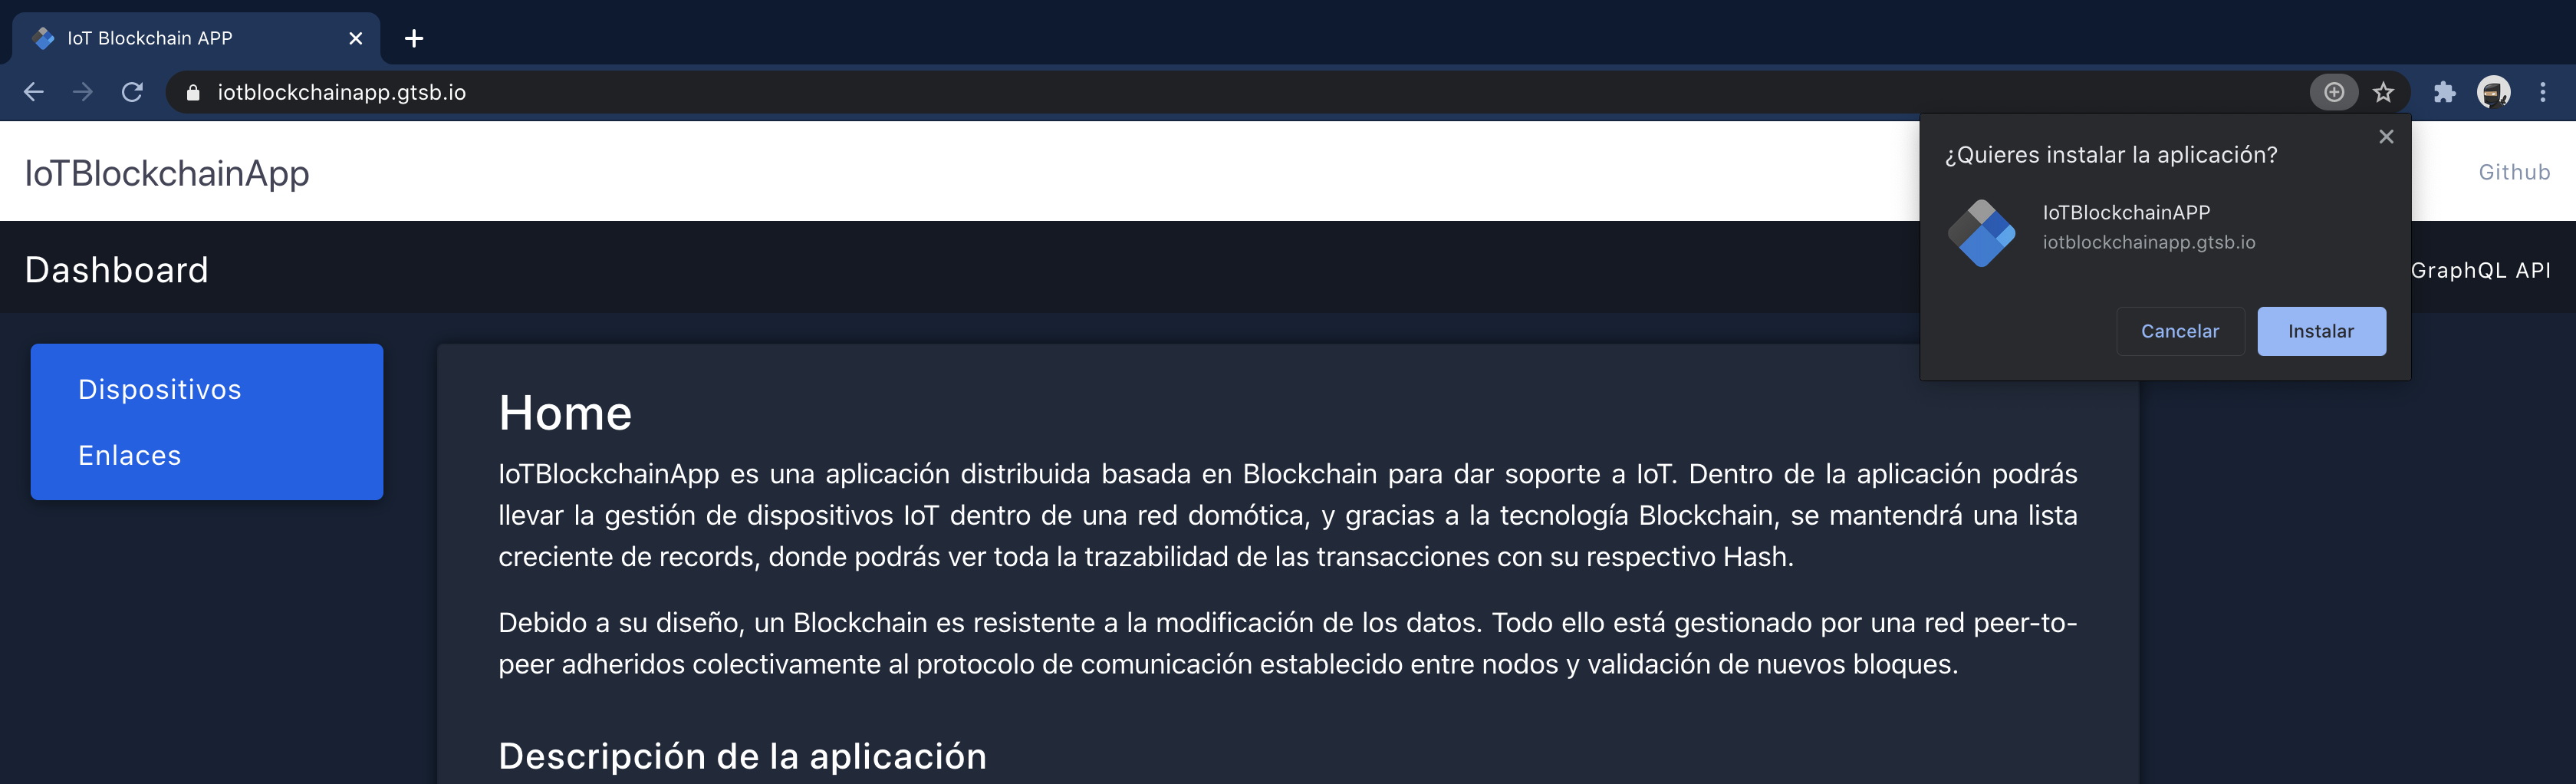
\includegraphics[width=10cm]{imagenes/desarrollo/web/pwa/instalacion_pwa_portatil}
  \caption{Instalación PWA en portatil.}
  \label{fig:instalacion-pwa-portatil}
\end{figure}

\begin{figure}[ht!]
  \centering
  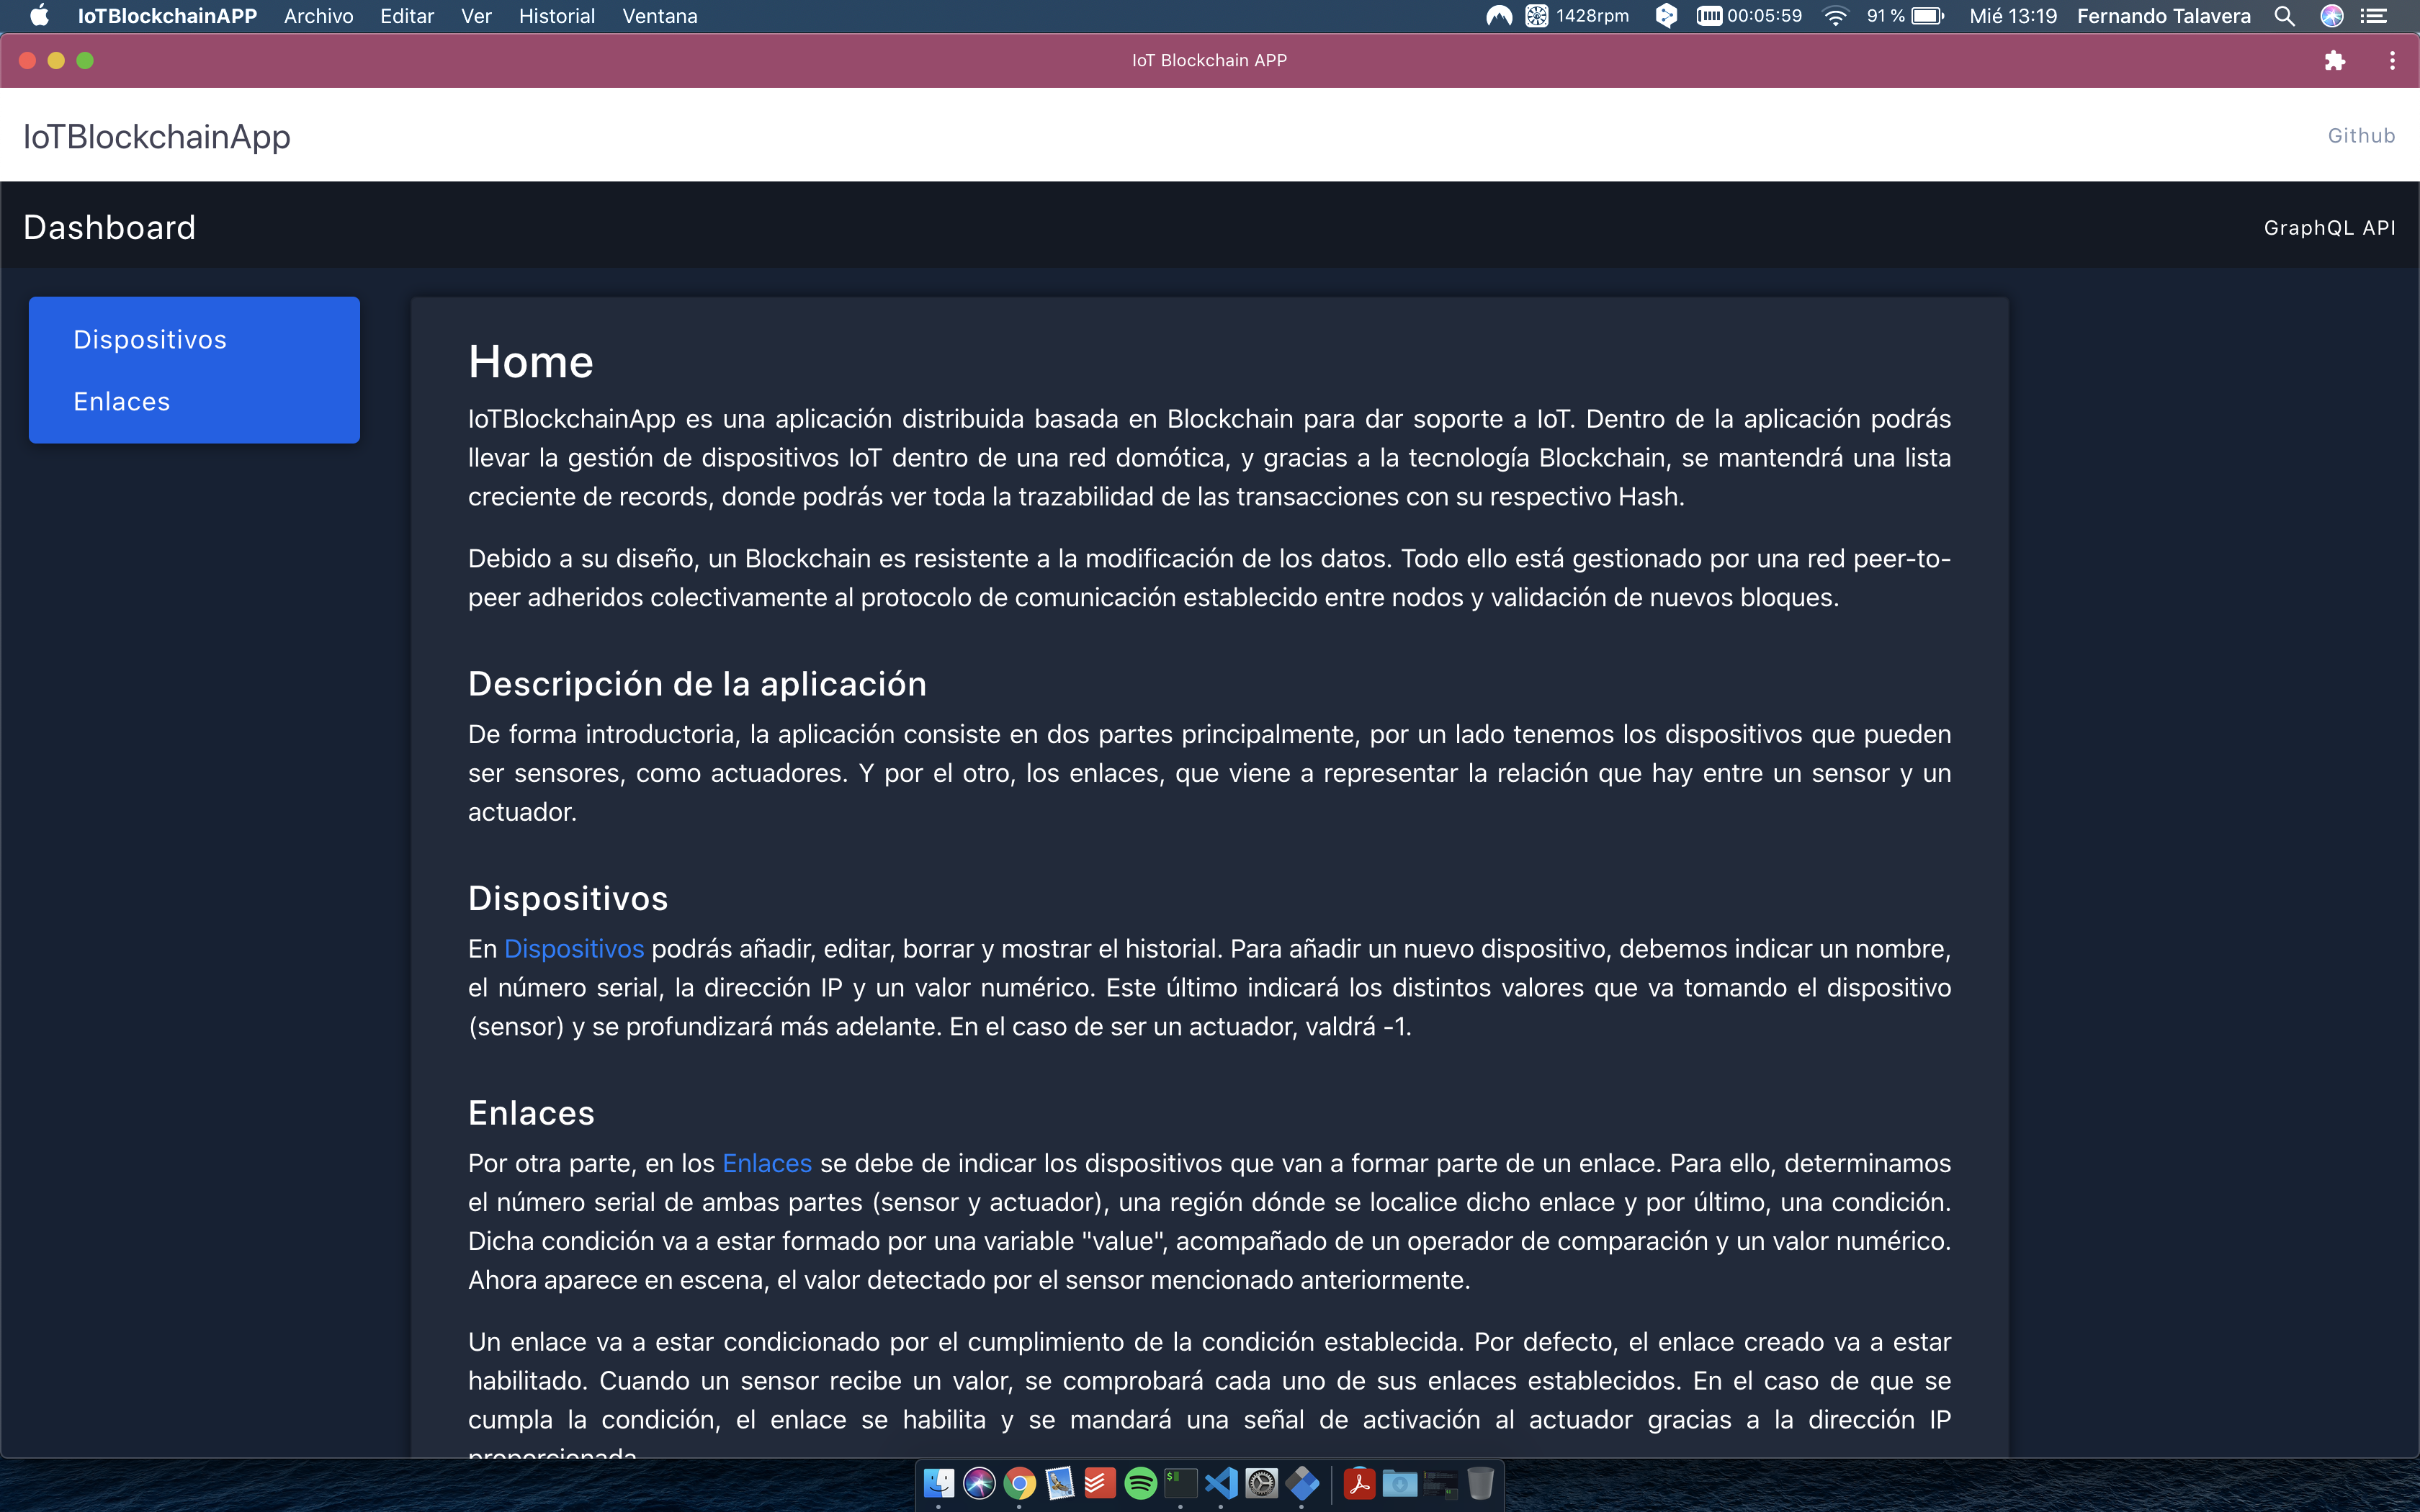
\includegraphics[width=10cm]{imagenes/desarrollo/web/pwa/app_portatil}
  \caption{App PWA en portatil.}
  \label{fig:app-portatil}
\end{figure}

\subsubsection*{Móvil.}

\begin{figure}[ht!]
  \centering
  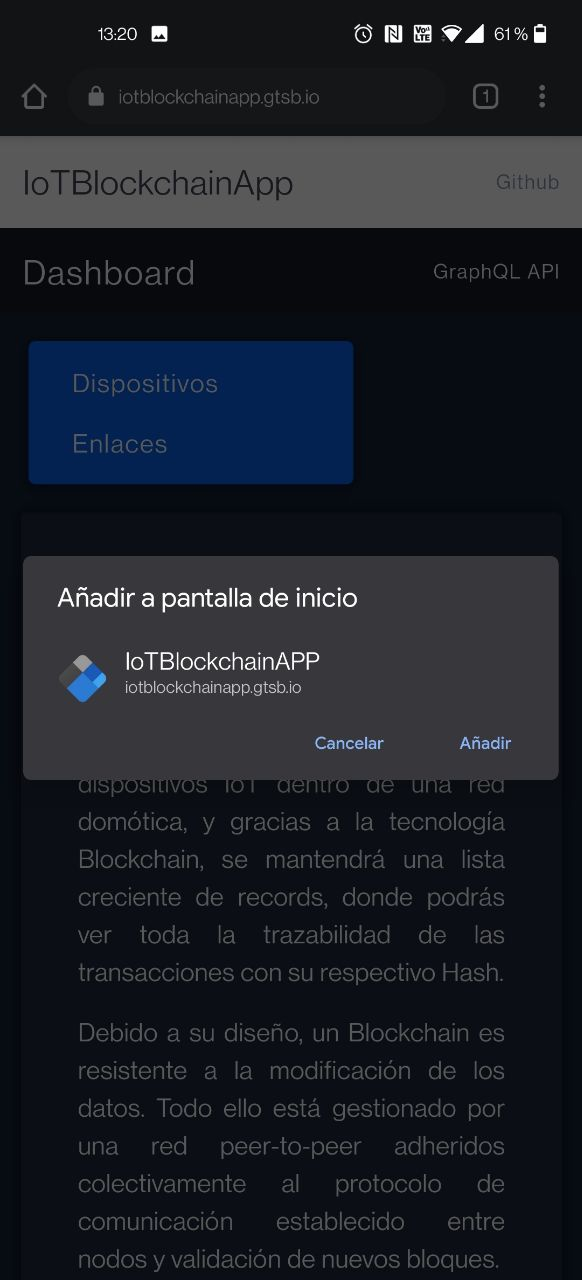
\includegraphics[width=10cm]{imagenes/desarrollo/web/pwa/instalacion_pwa_movil}
  \caption{Instalación PWA en móvil parte 1.}
  \label{fig:instalacion-pwa-movil1}
\end{figure}

\begin{figure}[ht!]
  \centering
  
\includegraphics[width=10cm]{imagenes/desarrollo/web/pwa/instalacion_pwa_movil2}
  \caption{Instalación PWA en móvil parte 2.}
  \label{fig:instalacion-pwa-movil2}
\end{figure}

\begin{figure}[ht!]
  \centering
  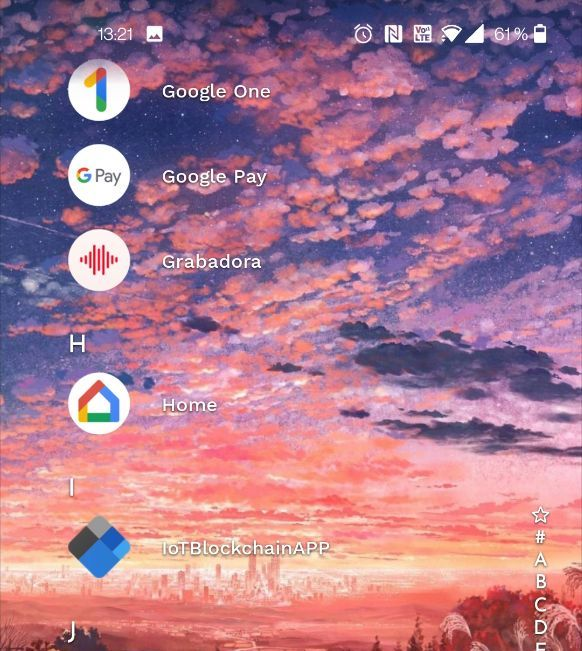
\includegraphics[width=10cm]{imagenes/desarrollo/web/pwa/icon_app}
  \caption{Icono de la aplicación en el móvil.}
  \label{fig:icon-app}
\end{figure}

\begin{figure}[ht!]
  \centering
  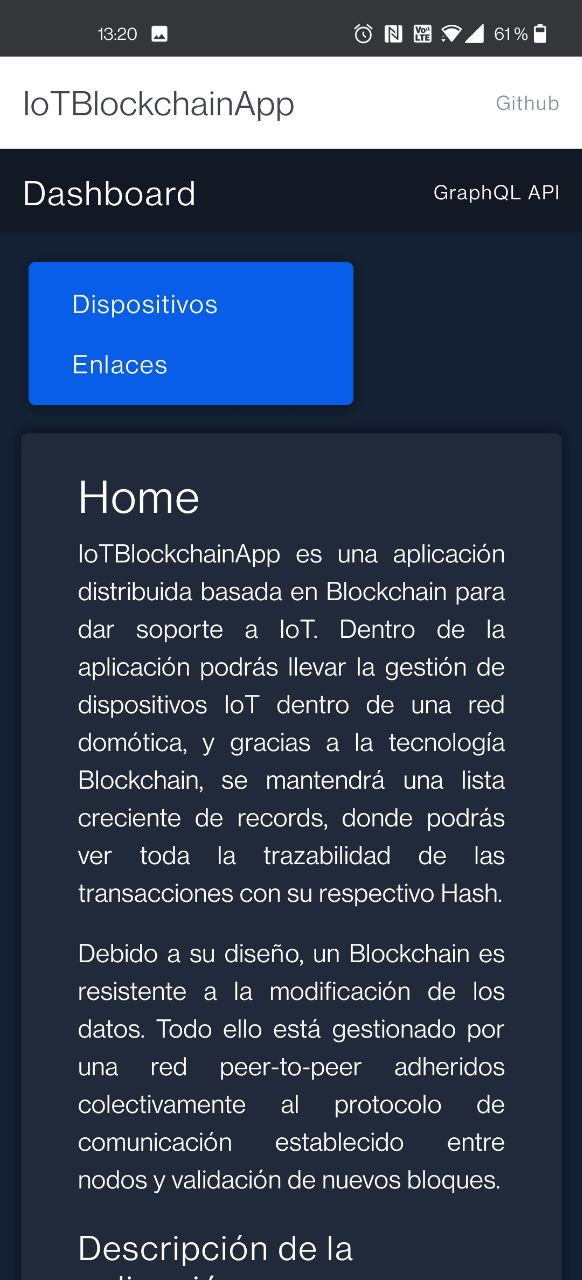
\includegraphics[width=10cm]{imagenes/desarrollo/web/pwa/app_movil}
  \caption{App PWA en movil.}
  \label{fig:app-movil}
\end{figure}

\newpage